\chapter{Game Design}
\label{chap:game_design}

\section{Obiettivo}
\label{obiettivo}

L’obiettivo del lavoro di Tesi è stato quello di portare un pubblico che non conosce la tematica, ma è abituato a determinati contesti, che dimostra un interesse, anche non spiccato, verso questo bagaglio culturale, a mostrare curiosità nei confronti del tema del pre-Cinema.

Il pubblico a cui si fa riferimento è quello di ragazzi tra gli 11 ed i 18 anni, frequentanti perciò la scuola media inferiore e superiore. Con lo sviluppo, negli ultimi decenni, di differenti tipologie di media e di canali di informazione, tale fascia di età risulta estremamente abituata a contesti ludici o altre definizioni di intrattenimento sviluppate in forma digitale.
Ogni scelta di design è stata perciò effettuata tenendo conto del pubblico fruitore del prodotto finale, cercando perciò di limitare l’uso di metafore di gioco, o meccaniche che potessero risultare troppo complesse per un pubblico giovane.
Nonostante i ragazzi in tale fascia di età abbiano mostrato familiarità con il mezzo videoludico, abbiamo notato varie capacità di approccio per quanto riguarda l’input e l’interfacciamento con il prodotto sviluppato. Abbiamo quindi ritenuto opportuno tener conto anche delle differenti abilità di gioco ed abitudini ad utilizzare differenti dispositivi di input, e di conseguenza a prendere delle scelte di design che fossero state coerenti con quest’aspetto.

Risulta importante specificare che l’obiettivo primario del lavoro non è stato quello di insegnare o inculcare concetti ai ragazzi fruitori del gioco. Un approccio del genere avrebbe portato il prodotto ad essere caratterizzato da una forma didascalica e didattica, che avrebbe rischiato di sortire persino l’effetto opposto nei confronti degli utenti del gioco, l’essere noioso e poco divertente, poco appetibile ad un pubblico giovane.
Si è data perciò particolare importanza alla scelta di meccaniche di gioco divertenti, ambientazioni che avessero generato curiosità e stupore ed un gameplay stimolante. Elementi accompagnati dalla possibilità di fruire di schede informative e contenuti inerenti la tematica che si è deciso di affrontare.

\subsection{Piattaforma di riferimento e momenti museali}
\label{sec:piattaforma_di_riferimento}

Una scelta cruciale nella produzione di una qualsiasi forma di videogioco, è quella relativa alle piattaforme per cui sviluppare il prodotto finale. Risulta evidente come tale scelta influenzi pesantemente ogni elemento di design, dalla caratterizzazione più o meno dettagliata delle ambientazioni all’interfacciamento dell’utente.

Una prima analisi è stata quella relativa ai momenti museali a cui poter far riferimento. Per momenti museali intendiamo gli intervalli temporali in relazione all’entrata del pubblico in museo:
\begin{itemize}
	\item \textbf{Pre-visita.} Sono quei momenti in cui il pubblico si incuriosisce riguardo l’ambito museale e si interessa di una possibile visita. Volantini, passaparola, pubblicità, sono elementi che influenzano e caratterizzano il momento della pre-visita.
	\item \textbf{Visita.}  È l’intervallo temporale che il pubblico trascorre all’interno del museo, viene caratterizzato perciò dai contenuti veri e propri, oltre che da tutti gli altri elementi presenti all’interno del museo.
	\item \textbf{Post-visita.} Sono i momenti successivi alla visita del museo. Sono direttamente correlati alla soddisfazione provata dal pubblico, che può consigliare la visita ad altre persone, oltre che svolgere attività coerenti al contesto museale e provare interesse nei confronti di ciò che ha visitato.
\end{itemize}
Si è innanzitutto valutata la possibilità di sviluppare un prodotto fruibile all’interno del museo. L’applicazione avrebbe perciò avuto lo scopo di accompagnare la visita, tramite dei piccoli giochi, che avrebbero permesso di osservare alcuni degli elementi, presenti all’interno del museo, da prospettive diverse, generando nel pubblico una maggiore curiosità riguardo argomenti che sarebbero potuti risultare noiosi o poco interessanti. Un prodotto con un simile approccio è naturalmente sviluppabile per dispositivi mobili.

Secondo una nostra ipotesi, avvalorata anche da una personale ricerca di mercato, applicazioni del genere risultano molto interessanti per fasce di età inferiori rispetto a quella di riferimento per il progetto di Tesi.
I bambini, infatti, risultano particolarmente attratti da applicazioni semplici, immediate e veloci che possono rendere più piacevole la visita al museo, anche in compagnia di amici.
Ci si è quindi concentrati nei due restanti momenti museali, quelli precedenti e successivi alla visita.

Risulta importante specificare che la scelta della piattaforma di riferimento è stata effettuata anche in base alle meccaniche di gioco che si sono delineate durante le fasi di design del gameplay.
Abbiamo valutato la possibilità di sviluppare un casual game per dispositivi mobili, ma tale scelta avrebbe portato ad un prodotto superficiale, che sarebbe potuto risultare troppo semplicistico per il tema da voler affrontare.

\begin{figure}%[h]
	\centering
	% left bottom right top
	%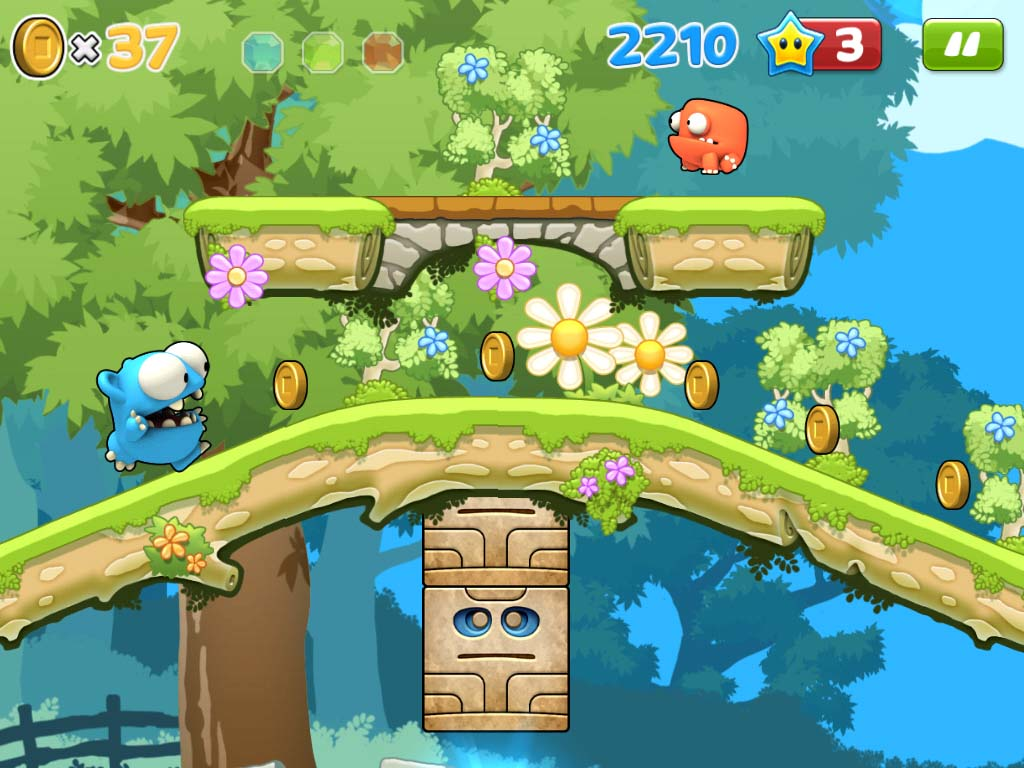
\includegraphics[clip= true, width= 0.8\columnwidth, trim= 1.5cm 3.0cm 0.6cm 0.0cm]{images/gameDesign/01_megarun.jpg}
	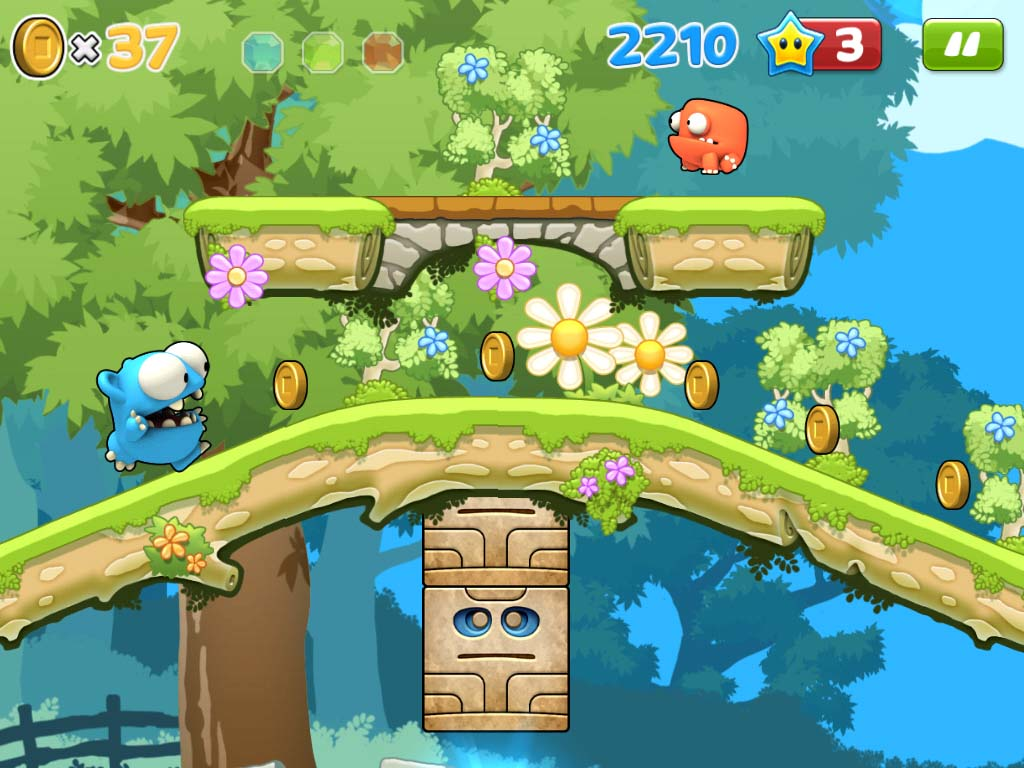
\includegraphics[width= 0.8\columnwidth]{images/gameDesign/01_megarun.jpg}
	\caption{Megarun: esempio di casual game.}
	\label{fig:casual_game}
\end{figure}

La natura platform/puzzle ideata durante le fasi di Design, ci ha spinto a sviluppare il prodotto per PC e console. Tali piattaforme permettono l’utilizzo di dispositivi di input più adatti alle tipologie di gameplay che sono state progettate, oltre che fornire una qualità visiva più consona all’estetica con cui si vuole caratterizzare il prodotto finito.
Tale scelta fornisce una ampia libertà di design, permettendo di sviluppare meccaniche complesse e profonde storyline, tipiche di una produzione di buon livello.

Concludendo, si è quindi scelto di sviluppare il videogioco per PC e console, con lo scopo di generare curiosità riguardo l’ambito del pre-cinema, attraverso meccaniche di gioco mirate, ambientazioni caratteristiche e schede informative studiate per fornire un buon supporto. Questo approccio risulta quindi coerente con i momenti museali di pre e post-visita, generando interesse nei confronti di un tema non ancora approfondito, o fornendo un buon metodo per osservare tematiche già note, apprese da una precedente visita, da un differente punto di vista.

\section{Meccaniche}
\label{sec:meccaniche}

Le meccaniche di gioco sono forse il nucleo più importante di una produzione videoludica di qualità, sono gli elementi che rimangono quando estetica, tecnologia e storia vengono meno, ed anche in queste condizioni, il prodotto, se caratterizzato da buone meccaniche, deve risultare piacevole ed efficace.
Il gameplay deve essere caratterizzato da regole semplici, ma allo stesso tempo flessibili, devono essere facili da capire, ma difficili da padroneggiare.

Il concetto di meccanica di gioco è strettamente legato a quello delle regole del game design, argomento che quindi non si limita ai videogiochi, ma a tutte le forme di intrattenimento che fanno riferimento al termine astratto di \textit{gioco}.
Abbiamo quindi fatto particolare attenzione al fornire al giocatore uno spazio di gioco in cui le meccaniche fornite avessero assicurato una sensazione di libertà, regolata però da limiti per circoscriverne le possibilità.
Il prodotto deve essere caratterizzato da pochi elementi di gameplay, ma che permettano al giocatore, entro certi limiti, di sentirsi libero di agire.

Ogni meccanica deve quindi essere semplice da capire e da utilizzare, ma deve richiedere un impegno ed uno studio progressivo per essere padroneggiata al meglio ed essere sfruttata in tutte le sue potenzialità.

Questo concetto è bene espresso nel libro \textit{The Art Of Game Design} \cite{artOfGameDesign}:
“Molti game designers sono d’accordo sul fatto che azioni interessanti che emergono col tempo siano la caratteristica di un buon gioco. Di conseguenza, il rapporto tra azioni significative e azioni di base è una buona misura di quanto un gioco emerga col tempo. Un gioco risulta elegante se permette al giocatore un piccolo numero di azioni di base, ma un grande numero di azioni significative.”

Chiaramente si tratta di un discorso soggettivo, ma ciò su cui abbiamo molto lavorato è stato trovare meccaniche di gioco semplici, ma che avessero permesso un vasto numero di possibilità in termini di level design e possibilità del giocatore.

\subsection{Elementi Platform}
\label{platform}
Il videogioco sviluppato presenta molte caratteristiche tipiche della categoria dei \textit{platform}.
Abbiamo scelto di utilizzare alcune meccaniche platform perché, oltre ad essere coerente con la rappresentazione che abbiamo deciso di creare durante le fasi di brainstorming, è un genere che sta tornando ad occupare una importante fetta di mercato. 

Il genere dei platform è nato nei primi anni ’80, ed ha avuto nel tempo una diffusione grandissima. Secondo wikipedia \cite{platform_wikipedia} , nel 1998 occupava il 15\% del mercato, nel 2006 ha avuto il suo massimo calo, arrivando ad occupare solo il 2\%, ma dal 2010 ha avuto una rinnovata popolarità, dovuta anche alla grande varietà degli endless runner che sono esplosi soprattutto nel mondo mobile. Anche la fervente attività degli sviluppatori indipendenti, sviluppatasi negli ultimi anni, ha fatto sì che il genere acquisisse di nuovo importanza nel settore. Tali studi, potendo contare su budget e mezzi limitati, hanno trovato, nel genere, un’importante base su cui poter costruire.

Per quanto riguarda il puro lato estetico, come mostrato in Figura~\ref{fig:platform_proportions}, il personaggio principale ha proporzioni non realistiche, molto accentuate in larghezza piuttosto che in altezza, con una proporzione che si avvicina all'1:1.

\begin{figure}%[h]
	\centering
	% left bottom right top
	%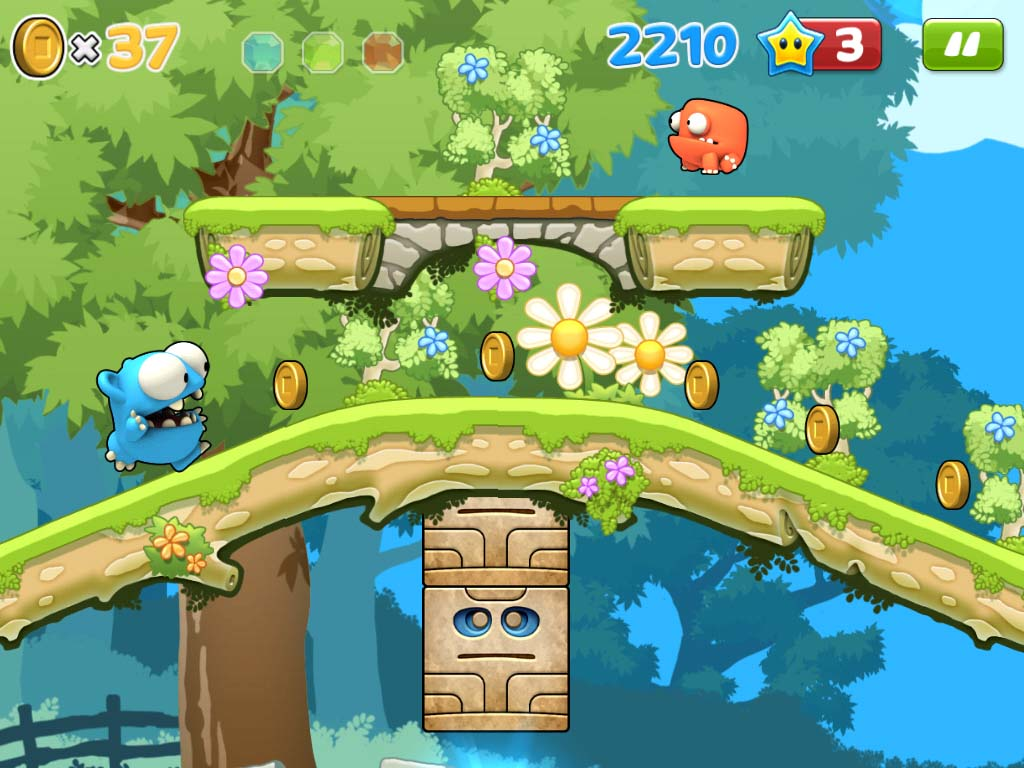
\includegraphics[clip= true, width= 0.8\columnwidth, trim= 1.5cm 3.0cm 0.6cm 0.0cm]{images/gameDesign/01_megarun.jpg}
	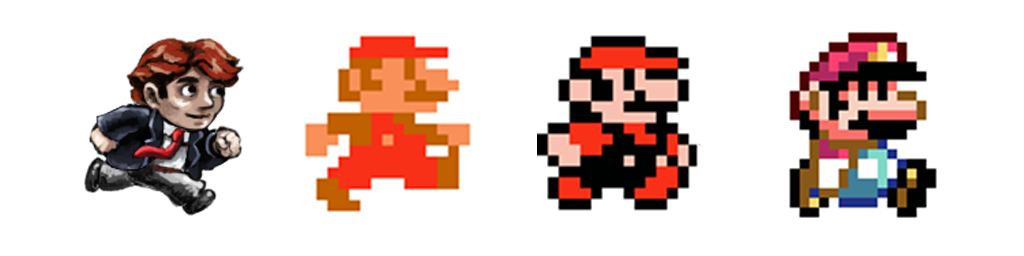
\includegraphics[width= 0.9\columnwidth]{images/gameDesign/02_braid_SM.jpg}
	\caption{Proporzione del personaggio di un platform game: Braid e SuperMario.}
	\label{fig:platform_proportions}
\end{figure}

Caratteristici dei platform sono quegli elementi di gioco che richiedono soprattutto delle abilità di reazione e concentrazione del giocatore, come corsa, salto o usare piattaforme.

Per quanto riguarda il movimento del personaggio, abbiamo deciso di ricorrere ad una corsa bidirezionale, a velocità uniforme in entrambe le direzioni ed indipendente dalla pressione del tasto di riferimento o dell’inclinazione della levetta analogica del controller. Questo assicura un padroneggiamento più veloce della meccanica, che, per le caratteristiche di gioco, non richiede una eccessiva complessità.
La velocità massima di corsa è raggiunta in maniera non esattamente istantanea, questo per assicurarsi un movimento non troppo brusco e quindi poco intuitivo.

La bidirezionalità fa sì che il personaggio si giri nel caso venga indicato un movimento opposto rispetto all’attuale direzione. Questo permette di raggiungere di nuovo, dove permesso dal design dei livelli, posti già visitati in precedenza (Figura~\ref{fig:platform_corsa}). Tale scelta non deve essere presa in maniera superficiale, in quanto ci si deve assicurare che elementi di gioco, incontrati in differenti momenti della partita, non si interfaccino in maniera problematica tra di loro. 
\begin{figure}%[h]
	\centering
	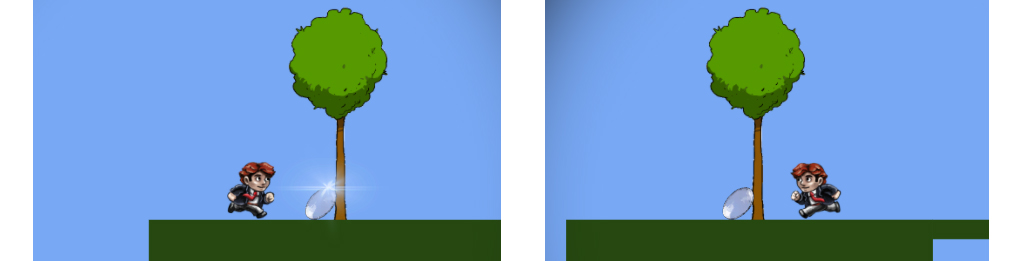
\includegraphics[width= \columnwidth]{images/gameDesign/03.jpg}
	\caption{Movimenti di corsa nel prototipo sviluppato}
	\label{fig:platform_corsa}
\end{figure}
In SuperMario Bros. (riferimento?) il personaggio può cambiare direzione, ma la camera non può tornare indietro, quindi, quando il personaggio arriva al bordo sinistro, è come se sbatta contro un muro invisibile.
La tipologia di gioco definita \textit{Endless Runner} invece, evita il problema impedendo al giocatore di invertire la direzione, nella maggior parte dei casi imponendo una corsa indipendente dall’input del giocatore o in altri casi semplicemente rallentabile o accelerabile (Figura~\ref{fig:platform_corsa_reali}).

\begin{figure}%[h]
	\centering
	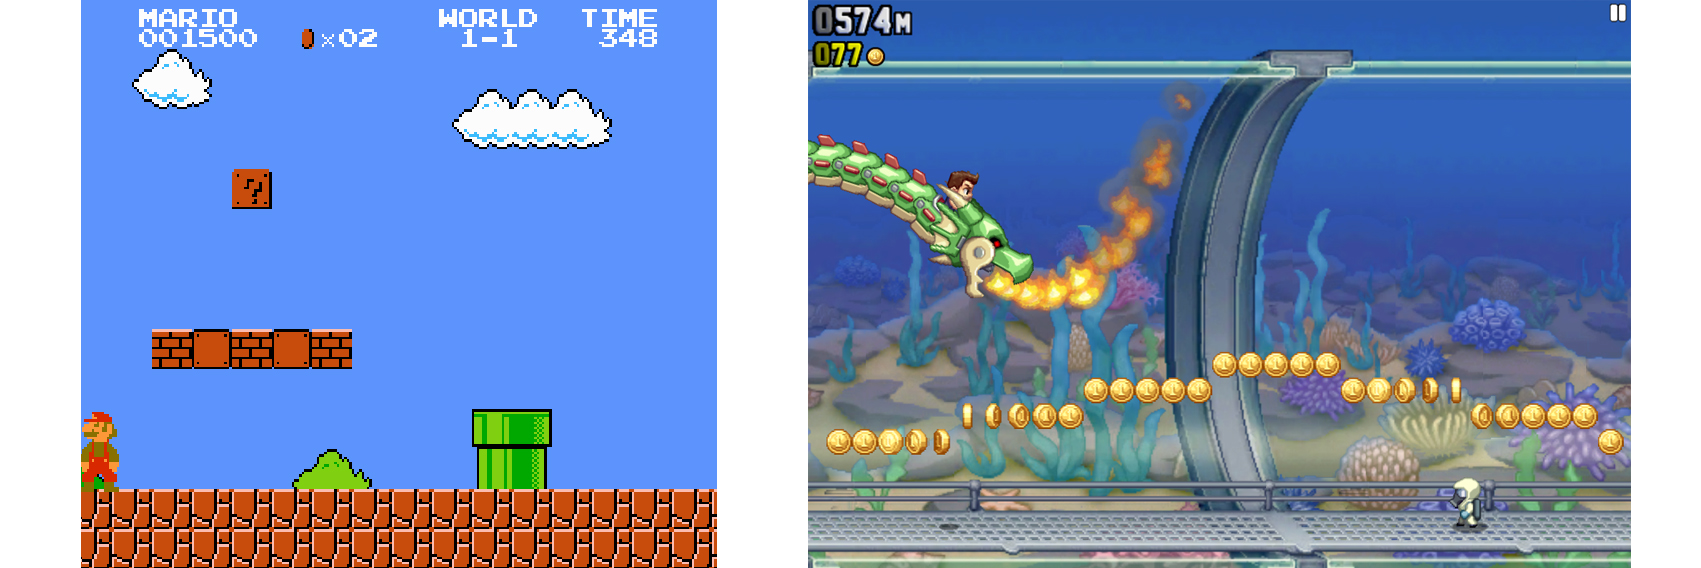
\includegraphics[width= \columnwidth]{images/gameDesign/04.jpg}
	\caption{Esempi di corsa: SuperMario e JetpackJoyride.}
	\label{fig:platform_corsa_reali}
\end{figure}

Per il salto, abbiamo deciso inizialmente di assegnare al personaggio una forza fissa verso l’alto, in seguito alla pressione del relativo bottone. Alcuni videogiochi invece assegnano una forza dipendente in maniera proporzionale dalla pressione del giocatore. Sono chiaramente due approcci differenti, il secondo fa sì che il salto sia una meccanica più complessa da padroneggiare, ma assicura delle possibilità di gameplay in più.
Durante i testing effettuati, abbiamo notato delle frequenti difficoltà nell’effettuare i salti, possiamo perciò pensare di prendere provvedimenti in tal senso, magari dando al giocatore un maggior controllo sulla potenza di salto, o limitando le sezioni in cui l’utilizzo del salto risulti troppo cruciale.

I movimenti del personaggio in aria sono controllabili attraverso i tasti direzionali. Perciò, dopo il salto o in seguito ad una caduta, il giocatore può direzionare o aggiustare la traiettoria di discesa. Non tutti i videogiochi platform assicurano tale comportamento, ma abbiamo ritenuto potesse essere utile per non frustrare eccessivamente il giocatore in seguito ad un salto non perfettamente calibrato al momento dello stacco.
La caduta del personaggio è soggetta ad una gravità 3 volte superiore al normale, è un elemento già presente in \textit{SuperMario} e ampiamente utilizzato nei giochi del genere per garantire una sensazione di repentinità al giocatore. La velocità di caduta è comunque limitata per garantirne il controllo.

\begin{figure}%[h]
	\centering
	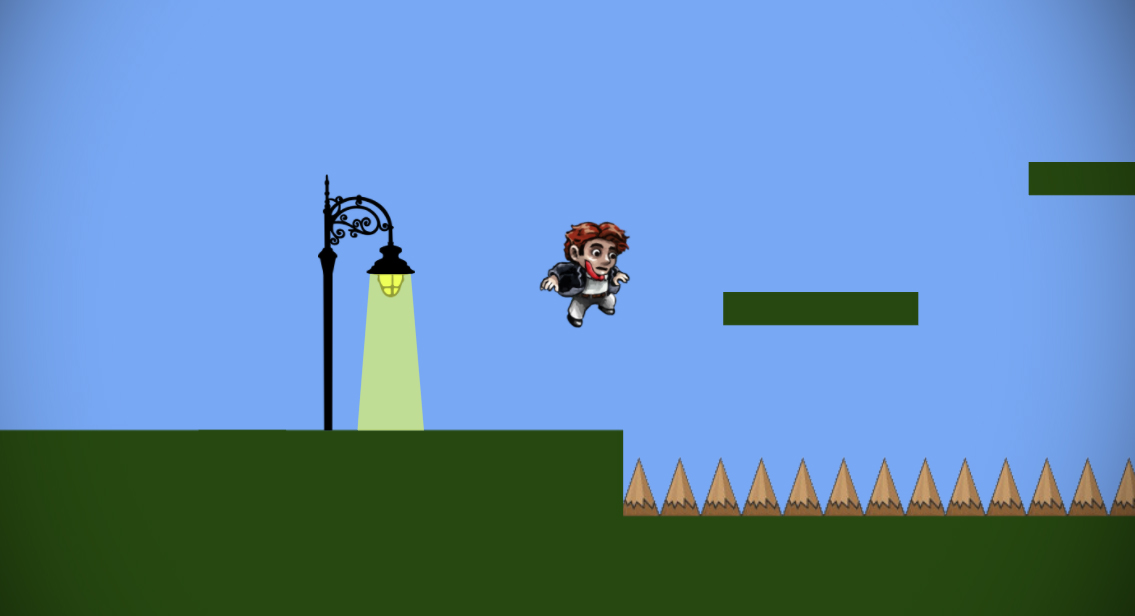
\includegraphics[width= 0.8\columnwidth]{images/gameDesign/05.jpg}
	\caption{Personaggio del prototipo, durante un salto.}
	\label{fig:platform_salto}
\end{figure}

Oltre alle meccaniche di corsa e salto, abbiamo dato la possibilità al personaggio di salire e scendere le scale. Questa è una meccanica non essenziale, che non aggiunge possibilità rispetto a quelle che non possa garantire una serie di salti, ma garantisce una maggiore sensazione di libertà al giocatore e permette una maggiore pulizia per quanto riguarda il level design. Le scale infatti, come mostrato in Figura~\ref{fig:platform_scala_piattaforme}, consentono di raggiungere luoghi per cui, altrimenti sarebbero state necessarie numerose piattaforme, che avrebbero potuto rendere la realizzazione dei livelli molto difficoltosa e confusa.

\begin{figure}%[h]
	\centering
	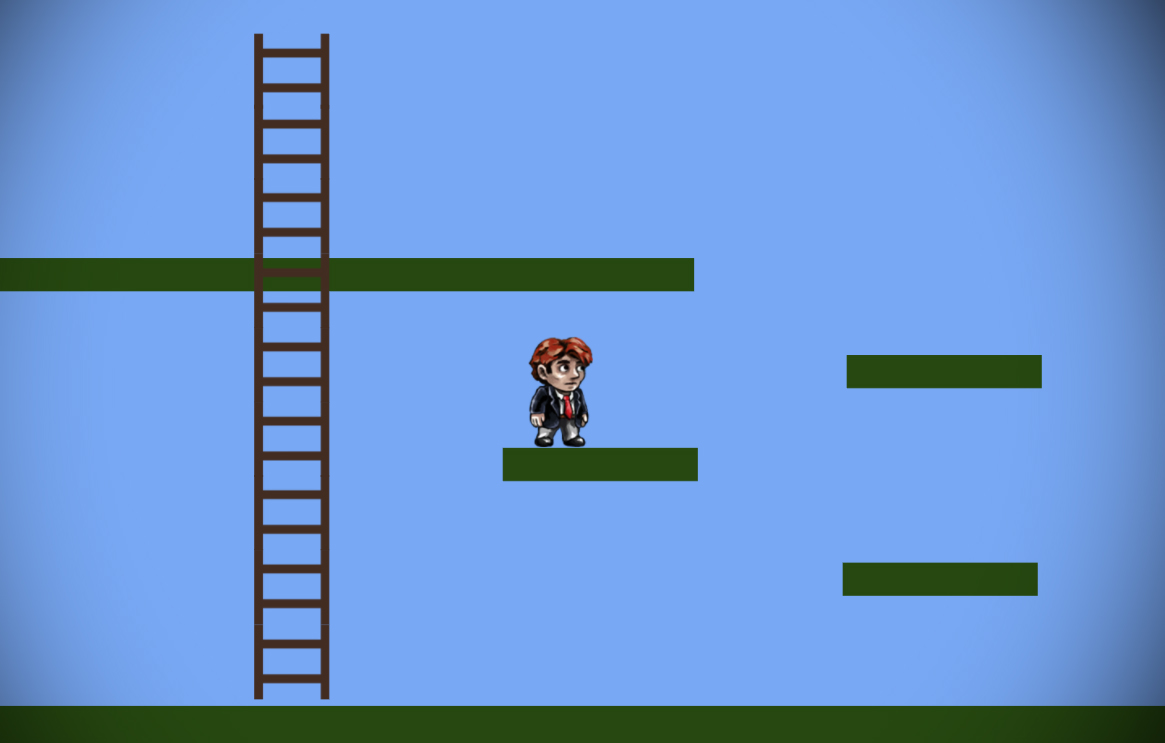
\includegraphics[width= 0.8\columnwidth]{images/gameDesign/06.jpg}
	\caption{Confronto tra utilizzo di scale e piattaforme equivalenti.}
	\label{fig:platform_scala_piattaforme}
\end{figure}

Le meccaniche di salto, controllo del personaggio in aria ed utilizzo scale sono state ispirate dal videogioco Braid (riferimento?), anche qui infatti il salto fornisce una forza indipendente dalla pressione del tasto e la possibilità di controllare il personaggio in caduta è una meccanica importante di gioco, anche se, rispetto a Braid, la forza impressa dal salto risulta meno forte e la gravità in caduta più espressiva, i movimenti in Braid appaiono più naturali, nel nostro caso invece più repentini ed eccessivi.

Sono state incluse nel gioco anche delle piattaforme mobili (Figura~\ref{fig:platform_piattaforme_mobili}). Queste hanno un movimento lineare tra due punti, uno dei quali raggiungibile dal personaggio, mentre l’altro si pone come obiettivo finale del movimento. Sono un elemento che mette alla prova le abilità di tempismo e di concentrazione del giocatore. Tali piattaforme risultano attraversabili dal basso verso l’alto, questo per permettere una maggiore libertà di approccio all’utente.
Durante i test effettuati, abbiamo notato che, spesso, i giocatori fanno fatica a comprendere i momenti esatti in cui la piattaforma cambia di direzione. Si sta perciò valutando se, nel prodotto finale non possa essere utile introdurre degli elementi che, graficamente, rappresentino dei limiti di inizio e fine corsa.

\begin{figure}%[h]
	\centering
	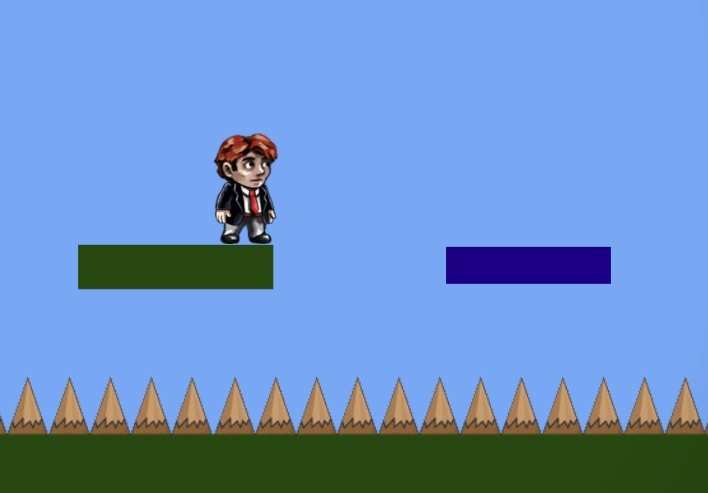
\includegraphics[width= 0.6\columnwidth]{images/gameDesign/07.jpg}
	\caption{Esempio di piattaforme mobili sviluppate.}
	\label{fig:platform_piattaforme_mobili}
\end{figure}

Graficamente, abbiamo deciso di rappresentare il terreno normale con una colorazione verde. Tale elemento non è attraversabile in nessuna direzione. Il personaggio collide sempre con esso.

Le piattaforme mobili vengono invece rappresentate con una colorazione blu scura, come si può osservare in Figura~\ref{fig:platform_piattaforme_mobili}.

Un altro terreno, che abbiamo deciso di sviluppare, permette di essere attraversato in entrambe le direzioni, ma solo se il personaggio sta utilizzando una scala. Permette appunto di attraversare terreni normalmente non attraversabili, ma caratterizzati dalla presenza della scala. La colorazione per questo tipo di terreno rimane comunque quella verde. Abbiamo verificato, tramite test e prototipazione, che questa scelta non influisce sulla comprensibilità della meccanica, in quanto caratterizzata dalla presenza della scala.

Parallelamente abbiamo ritenuto necessario sviluppare una tipologia differente di terreno, che permette di essere superato dal basso, ad esempio con un salto del personaggio. Non è attraversabile dall’alto. Tale scelta apre la strada ad una nuova meccanica, in quanto realizza una via a “senso unico” che può essere utile in fase di level design. Questo terreno invece, è differenziato dal resto tramite una colorazione blu più tenue rispetto alle piattaforme mobili.

Le 3 tipologie di terreno possono essere osservate in Figura~\ref{fig:platform_terreni}.

\begin{figure}%[h]
	\centering
	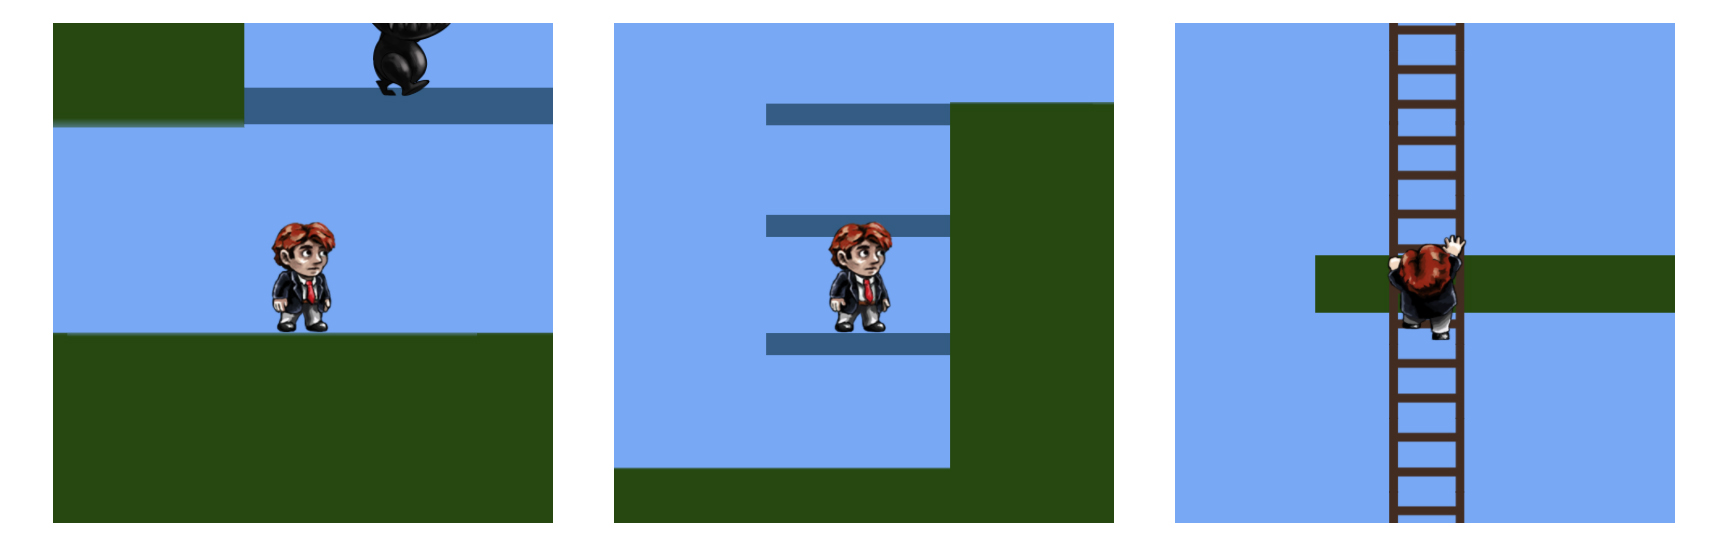
\includegraphics[width= \columnwidth]{images/gameDesign/08.jpg}
	\caption{Esempi delle tre tipologie di terreno sviluppate.}
	\label{fig:platform_terreni}
\end{figure}

\subsection{Elementi Puzzle}
\label{elementi_puzzle}

Oltre alle meccaniche Platform, che richiedono soprattutto reattività, tempismo e concentrazione del giocatore, il videogioco presenta anche caratteristiche tipiche del genere dei \textit{Puzzle Games}.

Questa categoria di videogiochi enfatizza soprattutto la risoluzione di enigmi e puzzles. Il giocatore deve perciò possedere le capacità di osservare la situazione in cui si trova il personaggio, analizzarne gli elementi, e capire in che modo debbano essere sfruttati ed usati per superare una determinata sezione o raggiungere un obiettivo.
Sono perciò richieste quelle che il libro \textit{The Art Of Game Design}\cite{artOfGameDesign} Definisce come abilità mentali (\textit{Mental Skills}):
“Le abilità mentali includono le capacità di memoria, osservazione e risoluzione di puzzle. Sebbene alcune persone evitino giochi che richiedono troppo impegno per quanto riguarda queste capacità, è raro che i giochi non le includano anche in piccola parte, perché i giochi sono interessanti quando ci sono decisioni interessanti da prendere, e prendere decisioni è una abilità mentale.”

Risulta necessario specificare che, nella fase di Level Design, abbiamo fatto particolare attenzione nel mescolare intelligentemente elementi platform e puzzle, in modo da essere in sintonia tra loro, senza che uno dei due elementi apparisse predominante sull’altro e che l’esperienza non risultasse eccessivamente frenetica e frustrante da un lato o lenta e noiosa dall’altro.
Le dinamiche puzzle ci hanno permesso anche di fare design riguardo il possibile utilizzo di strumenti particolari del pre-Cinema in maniera originale e curiosa (riferimento al capitolo), inserendo quindi elementi di gioco non presenti in altri esponenti del settore.
Elementi classici del puzzle game, che abbiamo inserito sono, ad esempio, leve, pulsanti, casse, porte, bilance e sequenze di bottoni.

Le leve (Figura~\ref{fig:platform_leve}) sono utilizzate per avere un effetto diretto sullo scenario di gioco. Generalmente, le abbiamo utilizzate per spostare elementi dell’ambientazione o attivare meccanismi.

\begin{figure}%[h]
	\centering
	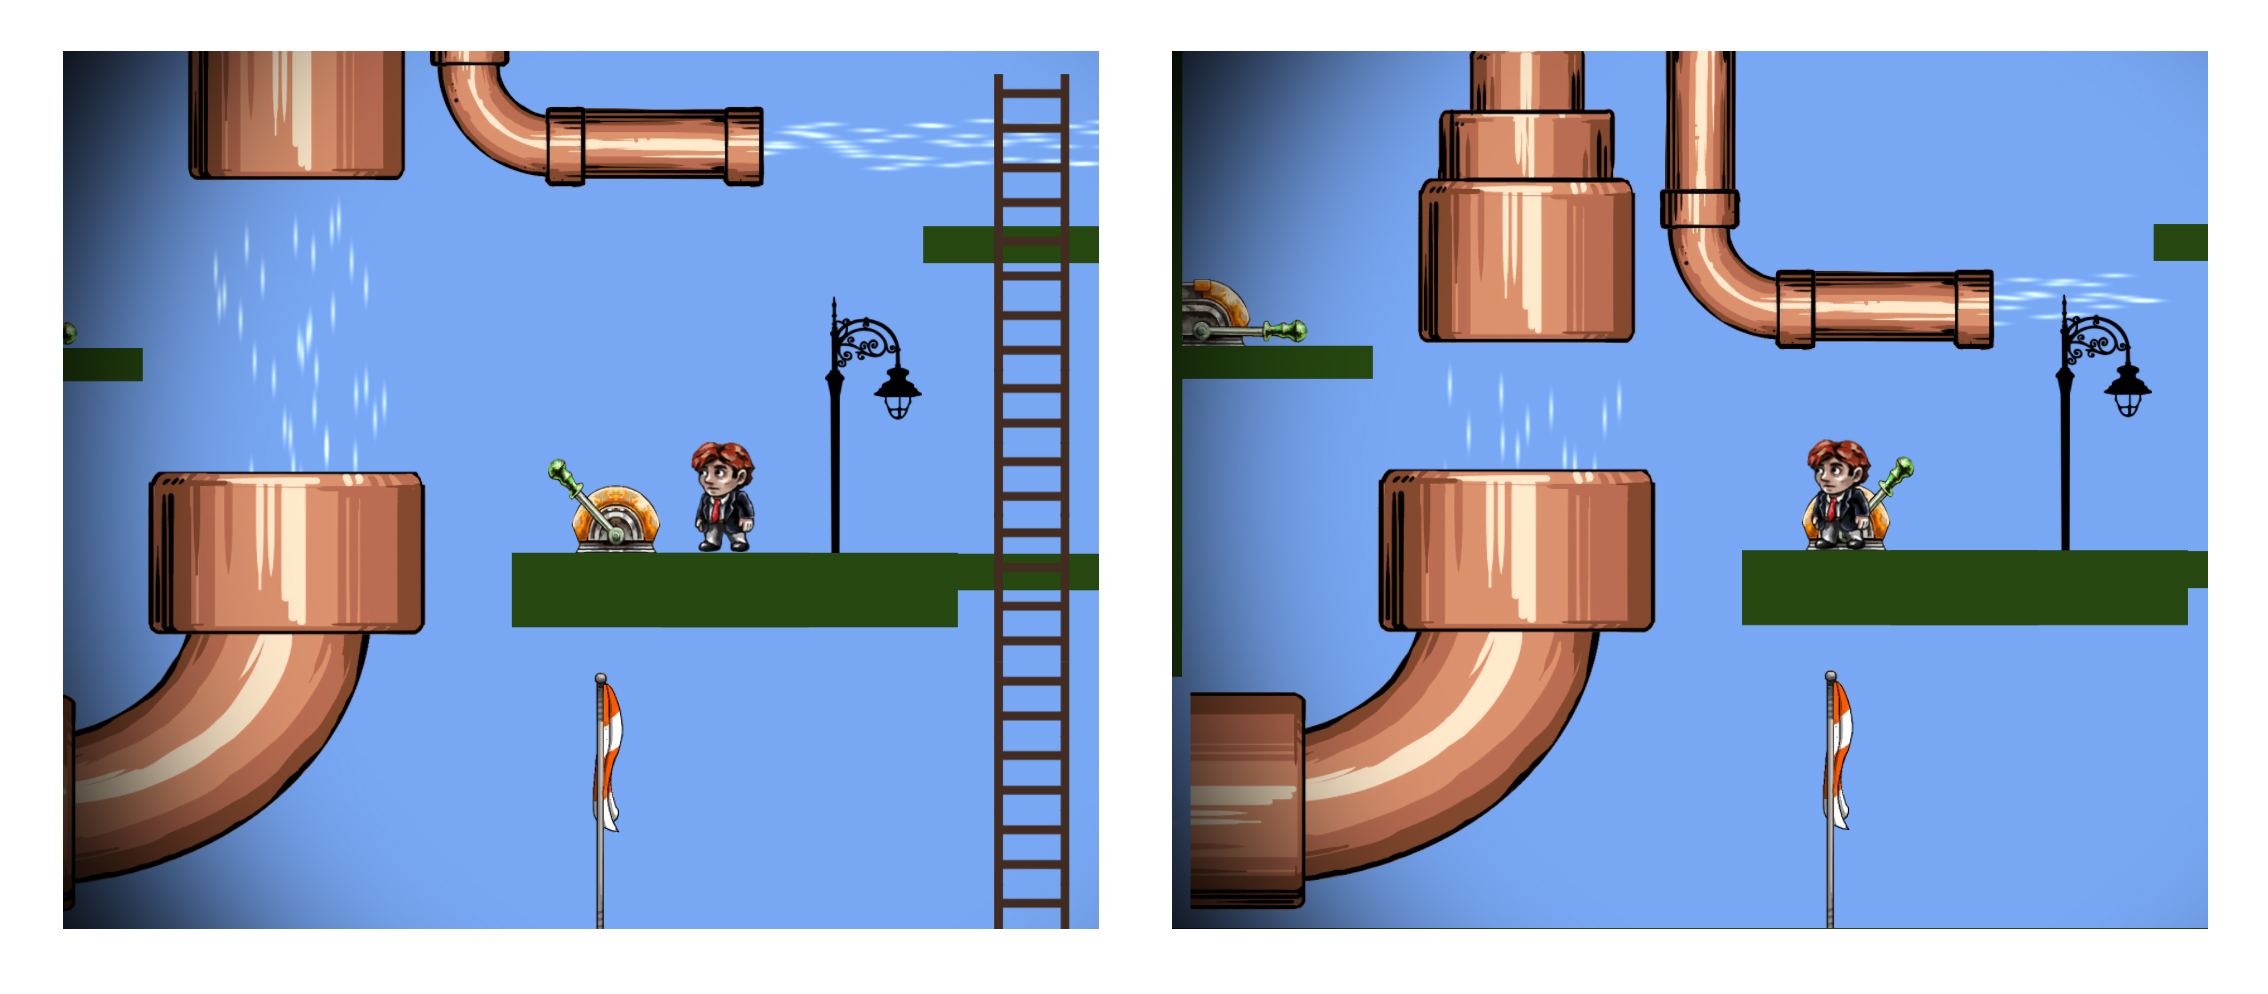
\includegraphics[width= \columnwidth]{images/gameDesign/09.jpg}
	\caption{Esempio di leva. Utilizzata per interagire con un elemento dello scenario.}
	\label{fig:platform_leve}
\end{figure}

I pulsanti a pressione possono essere intesi, concettualmente, come le leve, hanno un effetto immediato su alcuni elementi dello scenario. Nel nostro caso in particolare, abbiamo preferito associarli ad aperture e chiusure di porte, portoni o elementi traslabili che impediscono o permettono il passaggio del personaggio da una zona all’altra di gioco. Questa scelta è stata fatta per permettere al giocatore di capire immediatamente l’effetto di un bottone, spesso anche prima di premerlo.

L’attivazione dei bottoni avviene nel momento in cui il personaggio sale su di essi, hanno perciò un funzionamento a pressione. L’effetto diretto avviene al momento dell’attivazione. Quando il personaggio scende, i bottoni possono disattivarsi e quindi invertire l’effetto sortito sullo scenario di gioco o rimanere attivi e mantenere l’effetto nel tempo. Tale scelta dipende dal particolare utilizzo e quindi da scelte di level design.

I bottoni, come già specificato, vengono attivati dalla pressione su di essi, sia che venga applicata dal personaggio principale, che da un nemico (riferimento al capitolo). Come mostrato in Figura~\ref{fig:platform_bottoni} abbiamo comunque ritenuto utile inserire delle casse come elemento di gioco. Esse permettono di premere i bottoni senza la presenza del personaggio, oltre che salirci sopra per raggiungere posti più elevati.

\begin{figure}%[h]
	\centering
	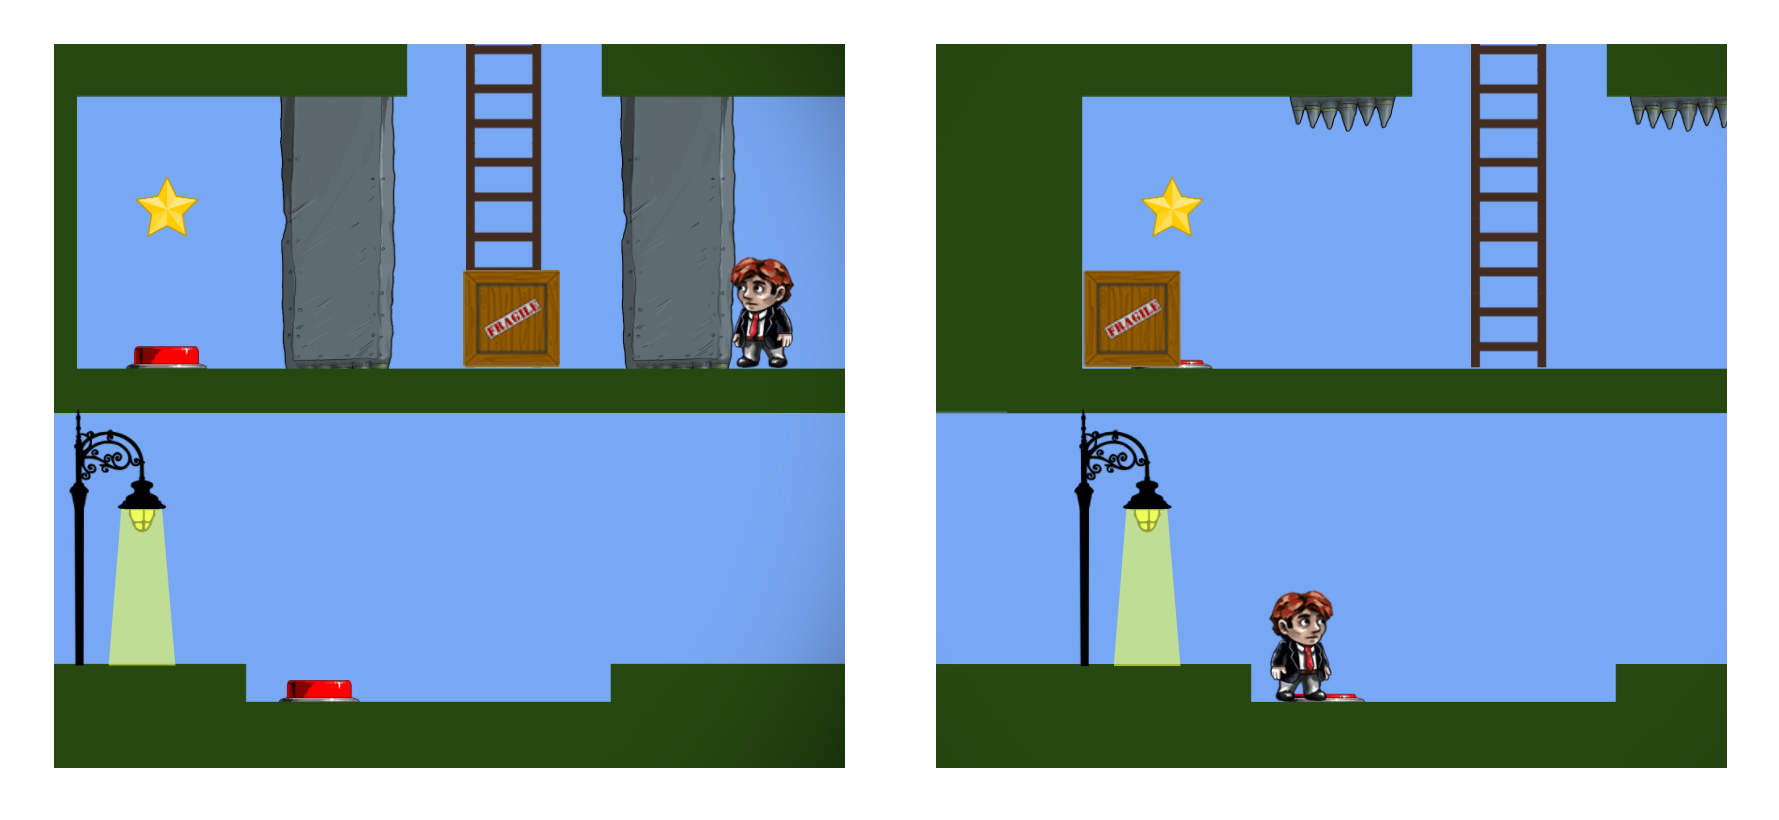
\includegraphics[width= \columnwidth]{images/gameDesign/10.jpg}
	\caption{Bottoni premuti dal personaggio e da una cassa.}
	\label{fig:platform_bottoni}
\end{figure}

Coerentemente con il concetto di pressione e pesi, abbiamo introdotto nel gioco anche delle bilance (Figura~\ref{fig:platform_bilancia}). Per semplicità, abbiamo ipotizzato che ogni elemento di gioco abbia una massa, relativamente alla bilancia, di una unità. Ipotizzando perciò che in un piatto ci sia una cassa, per avere una situazione di equilibro, è sufficiente che sull’altro piatto ci sia il personaggio. La bilancia, come le leve, permette di attivare un elemento dello scenario. È stata utilizzata, ad esempio, per un enigma in cui è necessario spostare un numero di nemici sufficienti in un piatto, per far sì che l’altro si alzi e attivi un bottone.

\begin{figure}%[h]
	\centering
	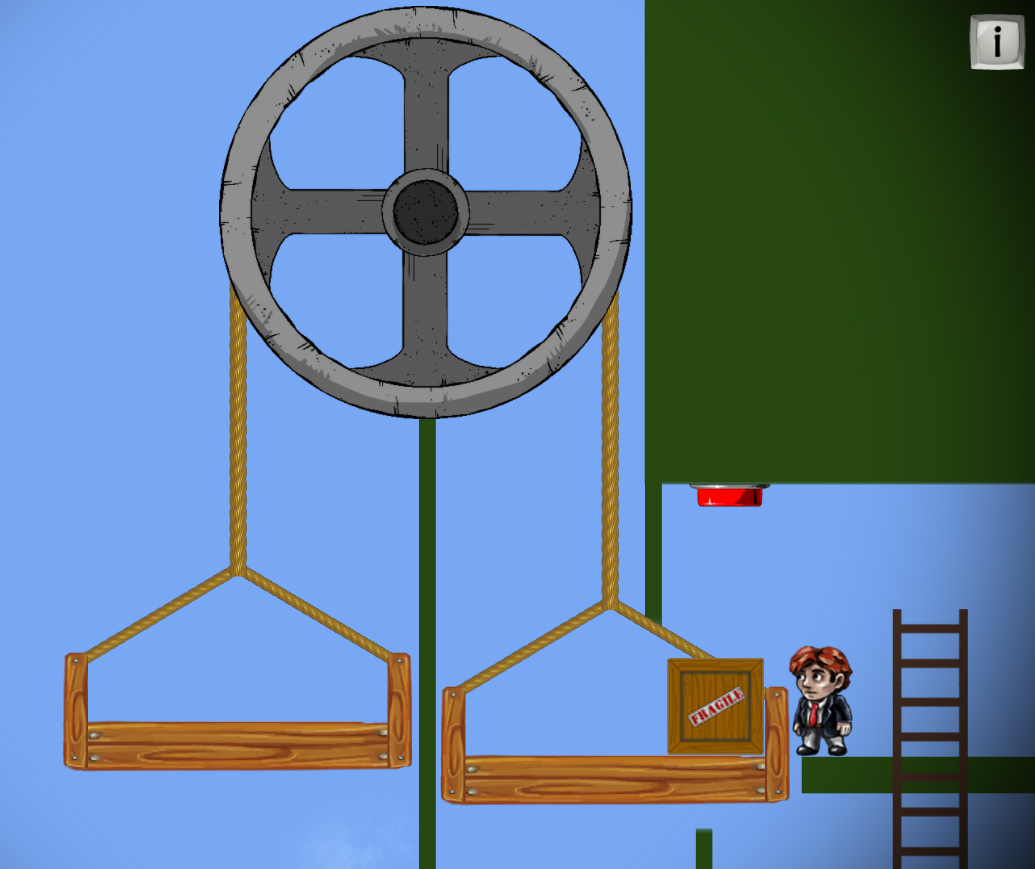
\includegraphics[width= 0.5\columnwidth]{images/gameDesign/11.jpg}
	\caption{Bilancia.}
	\label{fig:platform_bilancia}
\end{figure}

Un altro elemento interessante sono le sequenze di bottoni (Figura~\ref{fig:platform_sequenza_bottoni}
). Queste hanno lo stesso funzionamento dei bottoni singoli ma, per interagire con una porta è necessario attivarli tutti nella giusta sequenza. Se il primo bottone premuto è quello giusto, questo rimane attivo, se il secondo non è giusto, vengono disattivati tutti e la sequenza deve ricominciare dall’inizio. Quando vengono premuti tutti i bottoni nella giusta sequenza, viene attivato l’elemento dello scenario prestabilito, nel nostro caso le sequenze di bottoni sono sempre state utilizzate per aprire porte.

\begin{figure}%[h]
	\centering
	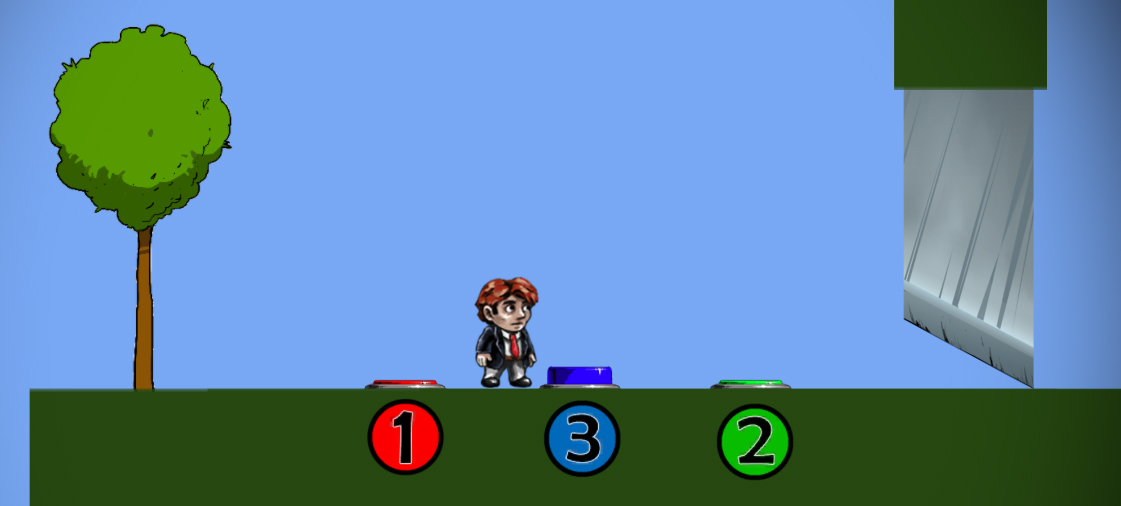
\includegraphics[width= 0.7\columnwidth]{images/gameDesign/12.jpg}
	\caption{Sequenza di bottoni.}
	\label{fig:platform_sequenza_bottoni}
\end{figure}

Viene riportata di seguito l’analisi di un enigma presente in uno dei livelli sviluppati. Nella figura \ref{fig:platform_enigma} si possono notare alcuni elementi non ancora analizzati, come il nemico, la lanterna magica o la stella, fare riferimento ai relativi capitoli (riferimenti) per approfondimenti sul loro utilizzo, che qui verrà spiegato in maniera superficiale.

\begin{figure}%[h]
	\centering
	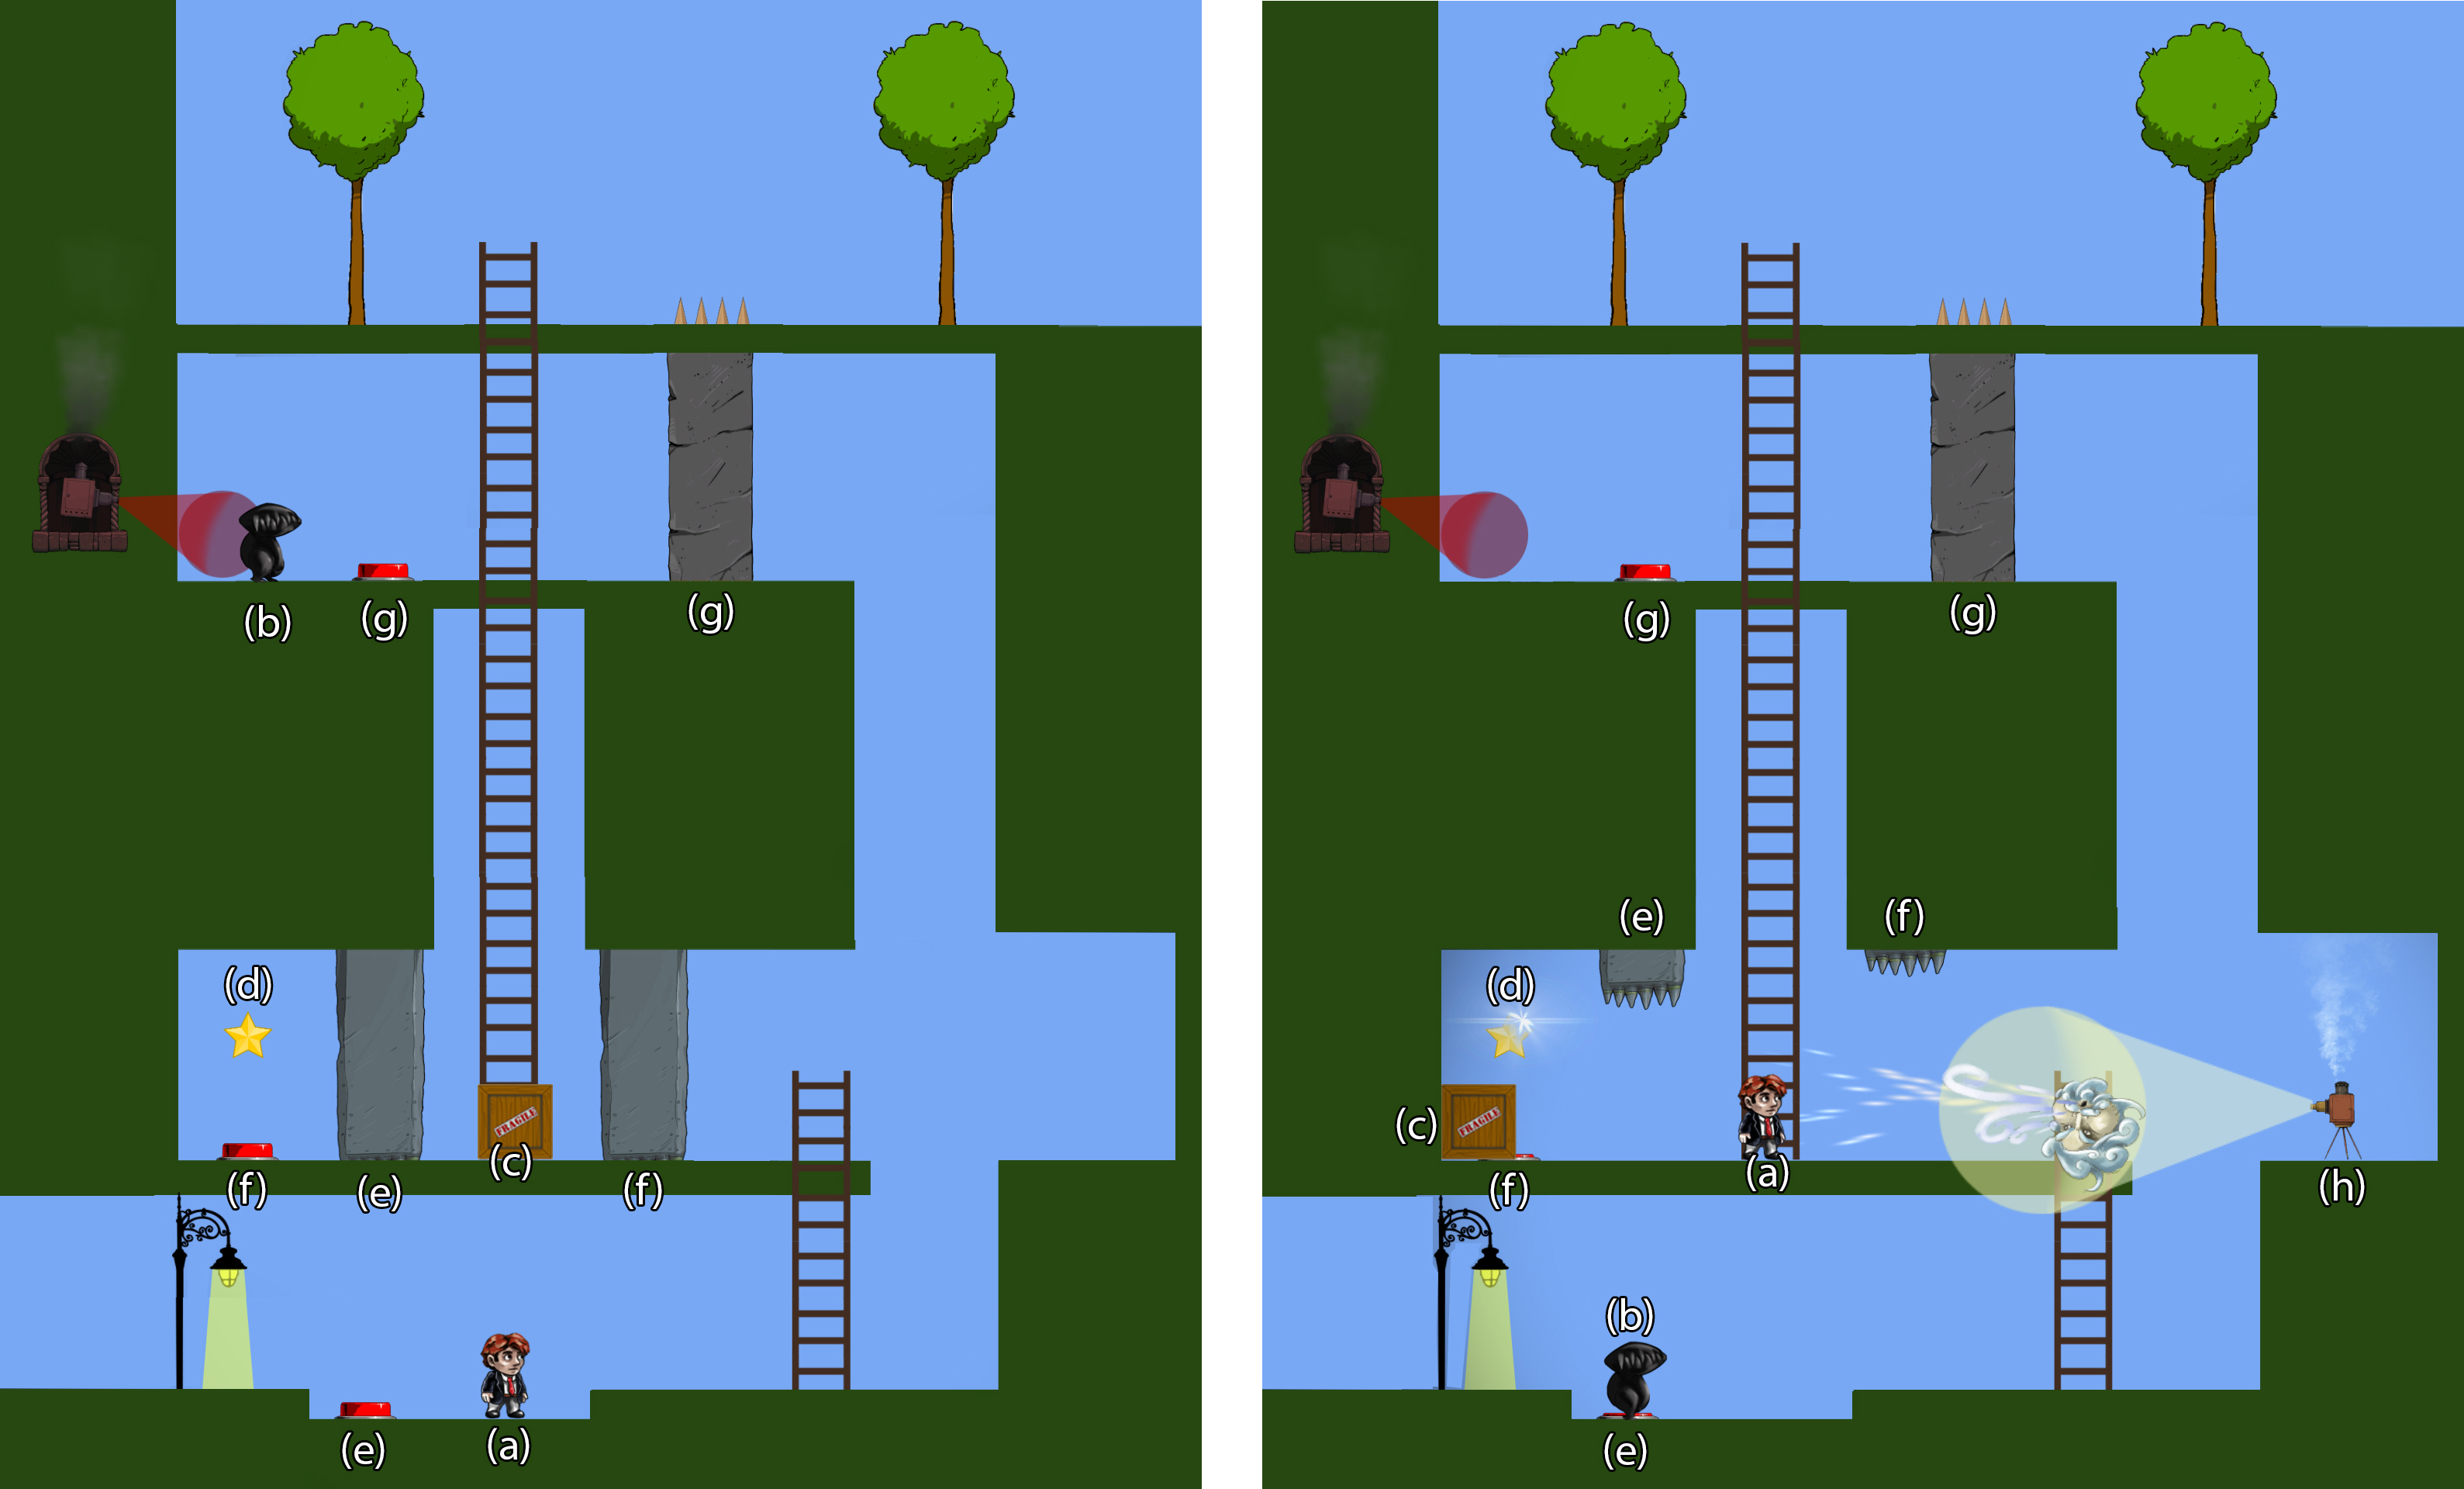
\includegraphics[width= \columnwidth]{images/gameDesign/13.jpg}
	\caption{Esempio di enigma.}
	\label{fig:platform_enigma}
\end{figure}

Come spesso avviene nei vari livelli sviluppati, la via per proseguire non richiede la completa risoluzione dell’enigma, ma solo la parte più semplice di esso, così da permettere, anche ai giocatori non interessati al raccoglimento di tutti i collezionabili, di proseguire con la partita.
In figura~\ref{fig:platform_enigma} vengono contrassegnati con la stessa lettera i bottoni e le relative porte che vengono azionate.

Il personaggio può subito porsi sopra il bottone “e” e notare l’apertura della relativa porta, che conduce ad una stanza con un altro bottone. Il giocatore capisce che la pressione di questo bottone è l’unico modo per proseguire. Raggiunge perciò un luogo favorevole per piazzare a terra la lanterna magica e sfruttarne il vento prodotto per spingere la cassa, bloccata però dalla porta “e”. Il personaggio deve quindi tornare sul bottone “e” e permettere alla cassa di premere il bottone “f”. Il personaggio può quindi raggiungere le scale e salire. Il nemico, premendo il pulsante “g”, attiva una porta con degli spuntoni, che blocca il raggiungimento dell’uscita, posta nella zona in alto a destra dell’immagine. Si deve perciò fare attenzione ad avere il giusto tempismo.

Come si può notare dall’immagine, il personaggio principale può quindi raggiungere l’uscita, ma rimane una stella da raccogliere. Come già specificato, solo la parte obbligatoria dell’enigma è stata risolta, ma non quella opzionale per il raccoglimento della stella.

Il giocatore può quindi, una volta salita la scala ed arrivati sul livello del nemico, scendere dalla scala, aspettare che il nemico si volti verso la porta/macigno, saltare il nemico, premere il bottone “b” e permettere così al nemico di cadere al piano inferiore. Questo, camminando, raggiungerà la zona con il bottone “e”, senza la possibilità di uscirne. Continuerà perciò ad attivare la porta che conduce alla stanza con la stella, che potrà quindi essere agilmente raccolta dal personaggio. Una volta collezionata, si può proseguire lungo il livello.
La seconda immagine in Figura~\ref{fig:platform_enigma} mostra l’enigma completamente risolto.

\subsection{Camera e Puntatore}
\label{sec:camera_e_puntatore}

Per quando riguarda la camera, abbiamo fatto in modo che questa fosse sempre approssimativamente centrata sul personaggio principale. In realtà usa una funzione che ne ammorbidisce il movimento, non segue perciò perfettamente il personaggio, ma tende in breve tempo alla sua posizione. Questa scelta è stata presa per rendere l’effetto meno brusco e quindi più gradevole alla vista.
Abbiamo anche ritenuto necessario includere la possibilità di evitare che la camera inquadri porzioni di scena non previste. È stata perciò valutata la capacità di gestire dei limiti della scena. Questa opzione è stata utilizzata solamente nel livello centrale, che funge da accesso agli altri livelli, ma sicuramente può fornire un mezzo ulteriore, in fase di design di altre meccaniche.

In seguito al design della meccanica di gioco principale, quella della Lanterna Magica (Riferimento), si è valutata la possibilità di inserire, per non confondere eccessivamente il giocatore, la possibilità di utilizzare un puntatore anche nelle normali fasi di gioco.

\begin{figure}%[h]
	\centering
	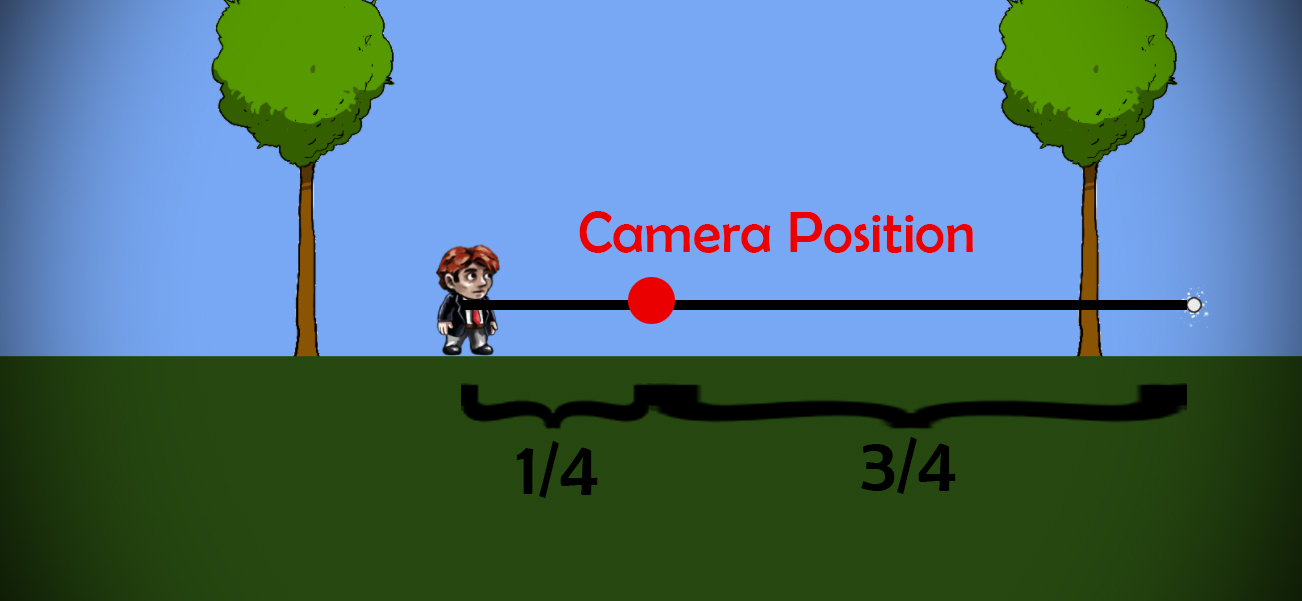
\includegraphics[width= 0.85\columnwidth]{images/gameDesign/15.jpg}
	\caption{Spostamento della camera in relazione alla posizione del personaggio e del puntatore.}
	\label{fig:camera_posizione_1_4}
\end{figure}

Il puntatore permette all’utente di spostare la camera dal personaggio principale ed osservare quindi porzioni di gioco che, normalmente, non sarebbero presenti nella visuale standard.
Il design del puntatore è stato un passaggio particolarmente difficile, che abbiamo perfezionato col tempo, in seguito allo sviluppo e test di vari prototipi.
Una delle prime versioni che abbiamo sviluppato, faceva tendere la posizione della camera al punto posto ad 1/4 del segmento che congiungeva il personaggio ed il puntatore, questo permetteva un allontanamento della camera dal personaggio, così da poter inquadrare una porzione di schermo maggiore (Figura~\ref{fig:camera_posizione_1_4}).

Ci siamo però resi conto che, nonostante l’effetto risultante fosse gradevole, l’utilità era particolarmente ridotta, in quanto non era possibile inquadrare elementi particolarmente lontani.
Si è perciò ipotizzato di allontanare la camera, lungo l’asse perpendicolare allo schermo, progressivamente con l’allontanarsi del puntatore dal personaggio.
In questo modo si è riusciti, con un effetto visivo di ridimensionamento degli elementi a schermo, ad inquadrare una porzione più grande di scena. Il maggiore problema riscontrato era comunque quello di un effetto forse troppo “pesante” all’occhio umano, che avrebbe perciò potuto generare confusione o addirittura fastidio al giocatore (Figura~\ref{fig:camera_allontanamento}).

\begin{figure}%[h]
	\centering
	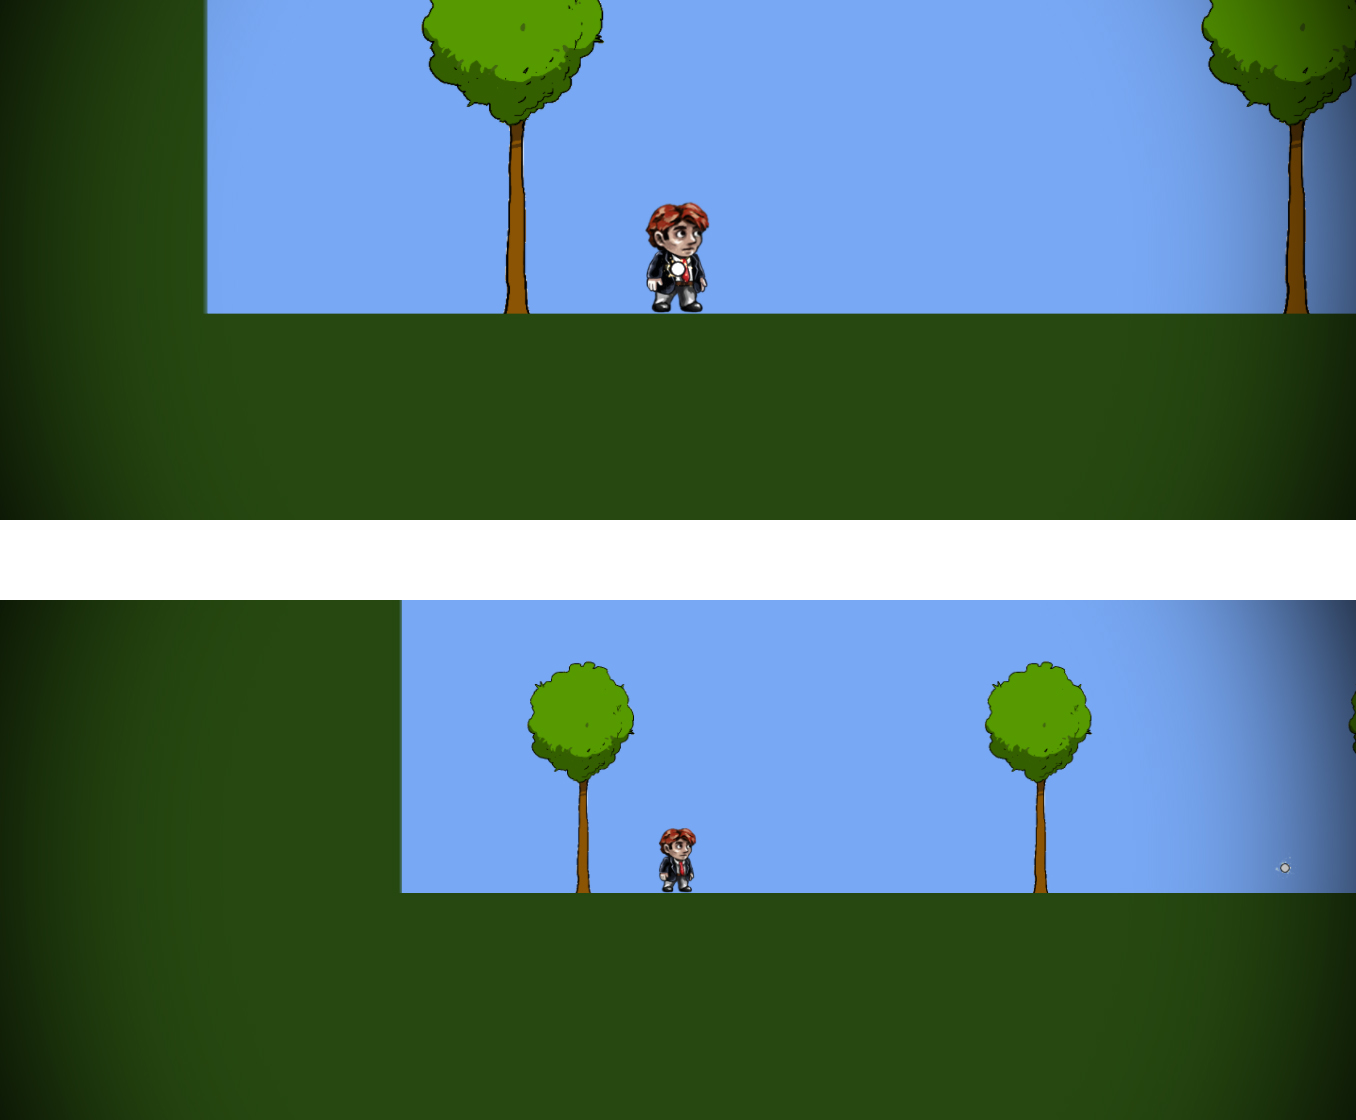
\includegraphics[width= 0.85\columnwidth]{images/gameDesign/16.jpg}
	\caption{Allontanamento della camera in relazione alla posizione del personaggio e del puntatore.}
	\label{fig:camera_allontanamento}
\end{figure}

Abbiamo ulteriormente accentuato l’effetto di disturbo provando ad applicare un approccio ibrido, limitando perciò l’allontanamento della camera, ma accompagnandolo da uno spostamento della camera lungo l’asse tra il personaggio ed il puntatore. È stata perciò scartato la possibilità di sfruttare entrambi gli approcci.

Concludendo le nostre analisi, abbiamo scelto di applicare il primo approccio proposto, spostando perciò la posizione della camera in un punto compreso tra il personaggio ed il puntatore, aumentando però il rapporto tra le due porzioni di segmento (0.37 anziché 0.25), così da poter inquadrare anche elementi più lontani. La camera raggiunge però tale posizione in un tempo particolarmente lento, così da ottenere un effetto più gradevole e spingere il giocatore a muovere il puntatore verso l’esterno dello schermo.

Il puntatore, graficamente, come è possibile vedere in Figura~\ref{fig:camera_posizione_1_4} e Figura~\ref{fig:camera_allontanamento}, è rappresentato come un semplice cerchio bianco, da cui parte un minimale effetto particellare, così da renderlo più visibile.
Abbiamo inoltre ritenuta valida la scelta di far girare il personaggio nella direzione del puntatore così che enfatizzi la metafora dell’elemento come modo per osservare altre porzioni di scena.

Mentre il personaggio è fermo, il puntatore rimane sempre visibile a schermo e la camera si adatta alla posizione di personaggio e puntatore, come analizzato nei precedenti paragrafi. In una prima versione sviluppata, il puntatore risultava essere sempre visibile, e con la camera che si muoveva di conseguenza. Successivamente abbiamo valutato la possibilità di far scomparire il puntatore in determinate situazioni, così da escluderlo dalla componente platform del gioco, che non richiede un'eccessiva osservazione di elementi non immediatamente visibili a schermo, ed associarlo invece maggiormente alla componente puzzle.
Quindi nel momento in cui il personaggio effettua un qualsiasi movimento, il puntatore scompare e la camera torna ad adattarsi, con un movimento molto lento, alla posizione del personaggio.
Il puntatore rimane visibile durante i movimenti del personaggio solamente se questo è mosso manualmente dall’utente, che vuole perciò continuare ad osservare la scena pur non rimanendo completamente fermo.
Abbiamo ritenuto che tali scelte di design, per quanto riguarda il puntatore ed il relativo movimento di camera, abbiano portato ad un buon risultato, che è stato sempre apprezzato durante le fasi di testing del prodotto.

\subsection{Meccaniche ispirate all'ambito del pre-Cinema}
\label{sec:meccaniche_precinema}

Ispirandoci all’ambito del pre-cinema e ad alcuni strumenti utilizzati nel contesto, abbiamo valutato la possibilità di includere elementi di gameplay atipici e che quindi avrebbero potuto colpire il giocatore per inventiva ed originalità.

La Lanterna Magica (riferimento) è stata scelta per costituire la meccanica innovativa più rilevante del videogioco. Considerando la sua capacità di creare immagini che al pubblico sembravano reali, abbiamo valutato la possibilità di fare in modo che il personaggio potesse plasmare il mondo a suo piacimento proiettando immagini.
La Lanterna Magica utilizza dei vetrini che vengono proiettati sulle superfici attraverso l’utilizzo di un raggio di luce. Tali vetrini spesso erano composti da più parti. Una delle prime meccaniche che abbiamo quindi valutato è stata quella di raccogliere, lungo un livello, dei frammenti di vetrino che avessero permesso, una volta ricomposti, di utilizzare la lanterna per uscire dal livello.
Tale elemento di gameplay però, avrebbe limitato l’utilizzo della Lanterna Magica esclusivamente all’ultima parte del livello, mettendone in secondo piano le potenzialità. Abbiamo perciò scartato questa ipotesi di utilizzo, nonostante in parte sia alla base dello sviluppo dell’hub centrale (riferimento).

\begin{figure}%[h]
	\centering
	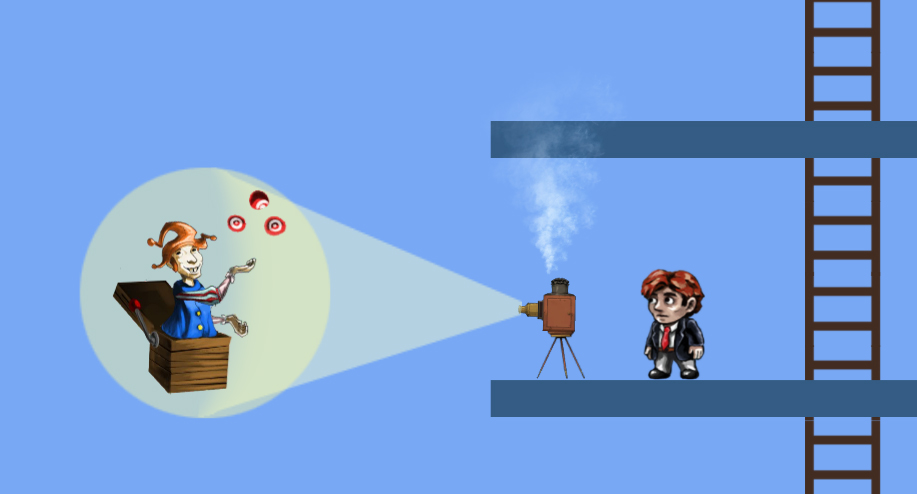
\includegraphics[width= 0.85\columnwidth]{images/gameDesign/17_giocoliere.jpg}
	\caption{Proiezione di Lanterna Magica.}
	\label{fig:meccaniche_precinema_lanterna01}
\end{figure}

Si è perciò valutata la possibilità di poter utilizzare in ogni momento la Lanterna Magica, magari dovendo raccogliere il vetrino da poter utilizzare lungo il livello. Si sono fatte alcune ipotesi per valutare le potenzialità di questo approccio, ed i risultati, ottenuti anche da alcuni test, sono subito sembrati molto promettenti.
Una delle iniziali idee proposte, è stata quella di usare due particolari proiezioni in grado di poter attirare (Figura~\ref{fig:meccaniche_precinema_lanterna01}) o spaventare i nemici, così da spingerli a svolgere determinate azioni o magari distogliere il loro sguardo dal personaggio.



È evidente come la lanterna magica sia uno strumento che, potendo proiettare nello scenario un qualsiasi tipo di elemento, apre le porte ad un amplissimo numero di possibilità di gioco.
Il passaggio successivo è stato quindi quello di cercare delle proiezioni che avessero permesso di avere meccaniche semplici da utilizzare, ma con un buon potenziale per lo sviluppo di sezioni ed enigmi di gioco. Tra quelle che abbiamo valutato ci sono, a titolo di esempio:

\begin{itemize}
	\item \textbf{Piattaforma.} Permette al personaggio di saltarci sopra per raggiungere posti non raggiungibili. È la forma più basilare di modifica all’ambiente. Aggiunge un elemento già esistente nello scenario, non richiede quindi uno sforzo di comprensione eccessivo. Può essere utilizzata anche come passerelle per un nemico.
	
	\item \textbf{Molla.} Una sorta di piattaforma potenziata. Permette di ricevere una spinta verso l’alto proporzionale all’altezza di caduta e perciò di raggiungere posti ancora più elevati. Apre alcune possibilità di gameplay ulteriori rispetto alla piattaforma, in quanto esiste anche la possibilità di raggiungere posti differenti a seconda dell’altezza da cui inizia la caduta sulla molla.
	
	\item \textbf{Fantasma.} Spaventa i nemici. Permette di distrarre i nemici dal personaggio, oltre che spingerli verso un possibile obiettivo (bottone da premere). Si è inoltre, coerentemente con questa proiezione, valutata la possibilità di inserire tipologie di nemici che avessero reagito in maniera differente alla visione del fantasma, come nemici corazzati che per lo spavento avessero perso l’armatura e quindi diventati vulnerabili.
	
	\item \textbf{Esca (giocoliere).} Il giocoliere era una proiezione utilizzata anche nei tipici spettacoli di lanterna magica dell’epoca, quindi aggiunge anche un elemento di coerenza storica. Può essere utilizzato con le stesse modalità del fantasma, cioè per spingere il nemico verso un possibile obiettivo dello scenario.
	
	\item \textbf{Acquario.} Inizialmente è stato pensato come elemento che può essere utilizzato per rallentare tutto ciò che ne passa attraverso. Una cassa in caduta può quindi essere rallentata per permettere al personaggio di svolgere altre azioni. Successivamente si è valutata la possibilità di usarlo come elemento capace di generare confusione in un nemico, attraverso correnti imprevedibili al suo interno.
	
	\item \textbf{Vento.} Genera un potente flusso di vento che interagisce con l’ambiente di gioco. Può essere usato per spingere il personaggio, per rallentare i nemici, per spostare elementi dello scenario o per interagire con meccanismi sviluppati appositamente (girandole che aprono porte, mongolfiere).
	
	\item \textbf{Gabbia per nemici.} Capace di intrappolare un nemico per un breve periodo di tempo.
	
	\item \textbf{Guardaroba.} Traveste il nemico da personaggio principale e viceversa, così da confondere il comportamento degli altri nemici.
	
	\item \textbf{Burrone con spuntoni.} Permette di uccidere i nemici.
	
	\item \textbf{Fiamma.} Permette di uccidere i nemici e di interagire con elementi appositi (palloncini).
	
	\item \textbf{Picchio di legno.} Permette di interagire a distanza con leve ed altri meccanismi.
\end{itemize}

Le precedenti proiezioni sono state valutate attentamente, cercando di prendere in considerazione tutte le possibilità di gameplay che avrebbero potuto originare.
Considerando anche la struttura generale di gioco ed il numero di livelli che abbiamo stimato fossero necessari per fornire un’esperienza sufficiente (riferimento), abbiamo deciso di utilizzare le proiezioni della piattaforma e del vento (Figura~\ref{fig:meccaniche_precinema_piattaforma_vento}), in quanto la prima risulta di facile comprensione ed utilizzo, mentre la seconda mostra le vere potenzialità della lanterna magica e gli effetti che questa può creare nello scenario di gioco.

\begin{figure}%[h]
	\centering
	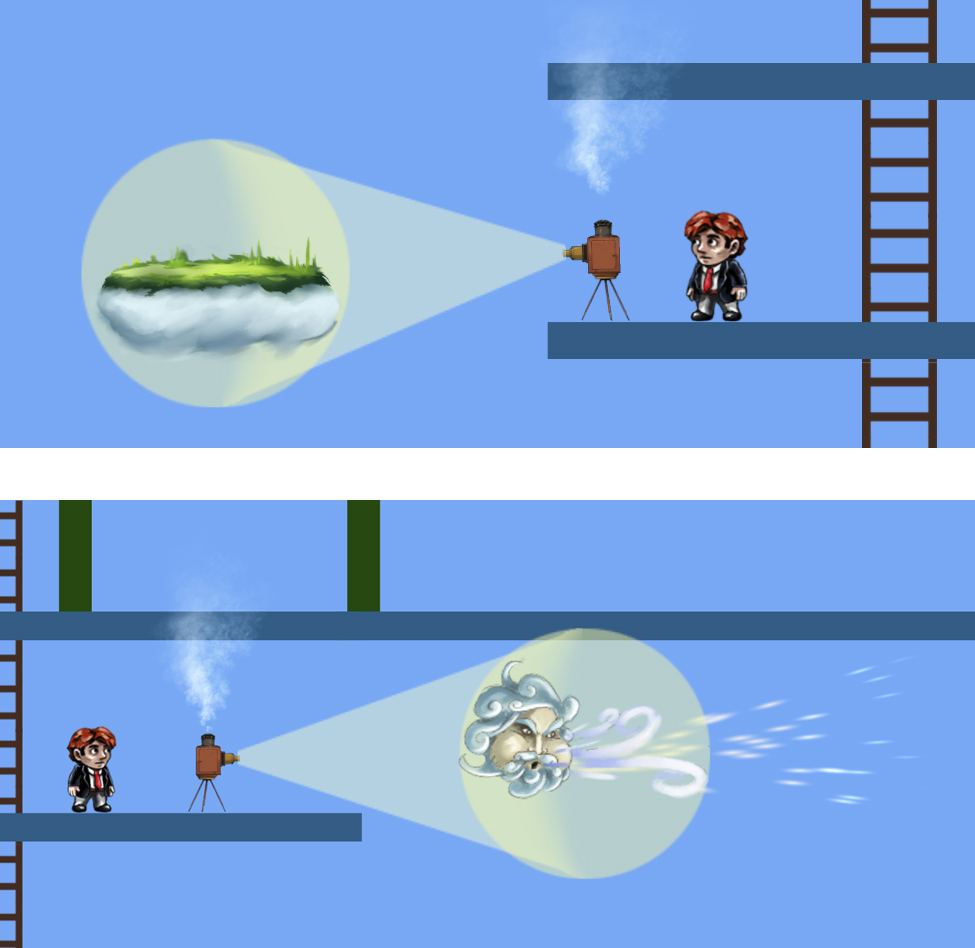
\includegraphics[width= 0.85\columnwidth]{images/gameDesign/18_piattaforma_vento.jpg}
	\caption{Proiezioni di vento e piattaforma.}
	\label{fig:meccaniche_precinema_piattaforma_vento}
\end{figure}

Per quanto riguarda la piattaforma, questa può essere attraversata dal basso verso l’alto, grazie ad un salto del personaggio, questo per evitare che il suo utilizzo non sia troppo complicato e l’operazione non risulti troppo frustrante. Come si può vedere in Figura~\ref{fig:meccaniche_precinema_piattaforma_vento}, abbiamo quindi deciso di renderla graficamente come una nuvola con, appoggiata su di essa, una porzione di terreno. Il giocatore ha quindi la sensazione di un terreno soffice, attraversabile, nella parte più bassa, mentre duro e concreto nella parte superiore.
Come già specificato, abbiamo utilizzato la piattaforma in quanto si tratta di un elemento di facile utilizzo e comprensione. Le piattaforme sono già presenti nello scenario di gioco, l’utente non si trova quindi spiazzato dalla sua presenza. Si trova però a dover ragionare sulla giusta posizione in cui porre la proiezione per far sì che questa sia di una qualche utilità.
Come verrà spiegato nell’analisi dei livelli (riferimento) si è preferito mostrare all’utente la lanterna e la relativa proiezione della piattaforma prima di dargli la possibilità di raccoglierla e quindi usarla. Questo per permettere un iniziale ambientamento del giocatore con la particolare meccanica di gioco e mostrare alcuni possibili utilizzi che potrebbero risultare poco intuitivi se richiesti direttamente all’utente.

La piattaforma viene utilizzata sia dal personaggio giocabile per raggiungere posti troppo lontani o per spostare nemici da una parte all’altra della scena, così da poter premere bottoni o interagire con l’ambiente nel modo previsto, come mostrato in Figura~\ref{fig:meccaniche_precinema_piattaforma}.

\begin{figure}%[h]
	\centering
	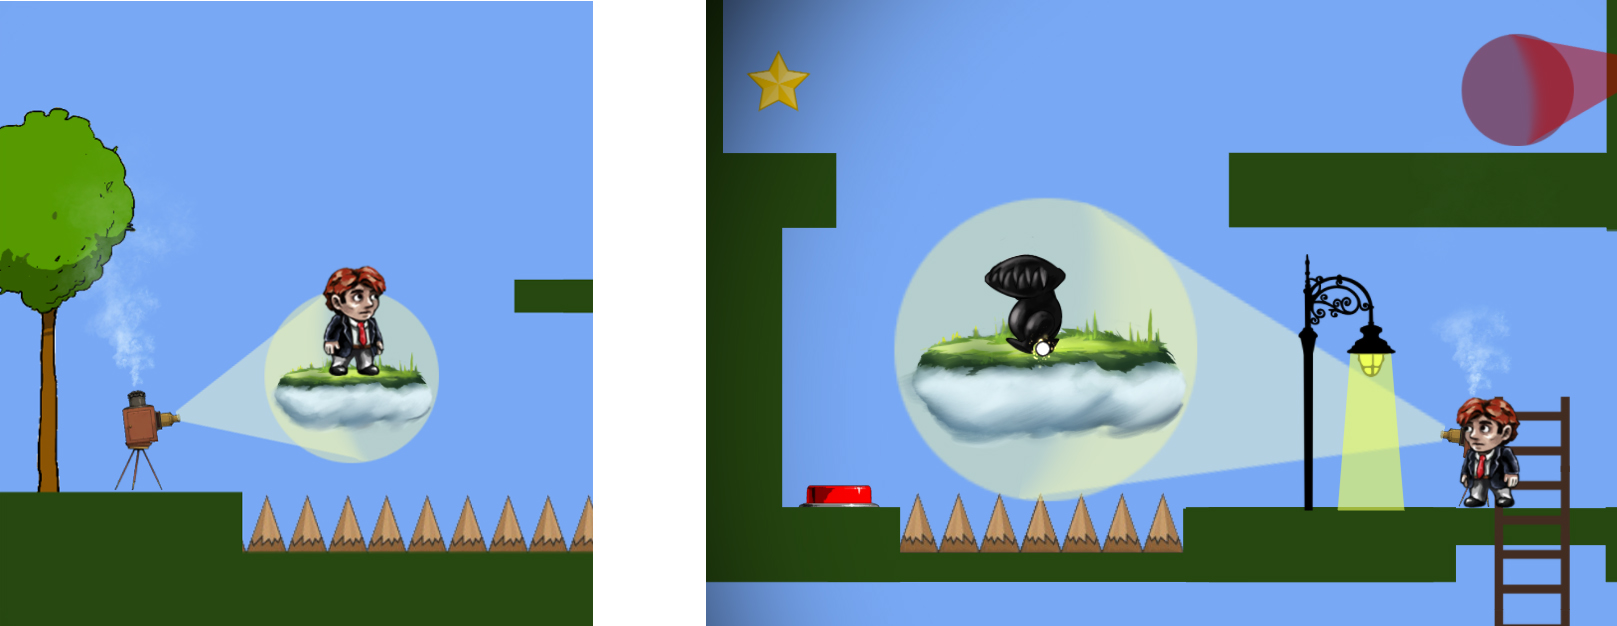
\includegraphics[width= \columnwidth]{images/gameDesign/19_piatt.jpg}
	\caption{Utilizzi della proiezione della piattaforma.}
	\label{fig:meccaniche_precinema_piattaforma}
\end{figure}

La proiezione del vento è invece caratterizzata dal fatto di interagire anche con l’ambiente e quindi non esclusivamente col personaggio di gioco. Gli alberi reagiscono al suo utilizzo, così come le foglie, le bandiere e le girandole presenti nel livello.
Come per la piattaforma, prima di permettere all’utente di usare la meccanica del vento, glie ne viene mostrato l’utilizzo in più forme.
Il vento può dare una spinta ulteriore al personaggio, permettendogli quindi di spiccare salti che possono coprire grandi distanze. Può quindi raggiungere zone molto elevate o saltare grandi burroni.
Tale proiezione può essere anche utilizzata per rallentare o velocizzare i nemici, a seconda del suo verso, per interagire con alcuni elementi dell’ambiente, sia in maniera puramente estetica, come i già citati alberi e bandiere, o per attivare meccanismi utili alla partita, come girandole che permettono l’apertura di speciali porte, mongolfiere con le quali è possibile raggiungere la cima di una montagna o barche a vela che permettono di superare distese d’acqua (Figura~\ref{fig:meccaniche_precinema_vento}).

Il vento è sicuramente una meccanica molto interessante, che esprime massimamente l’idea di sorpresa generabile da una proiezione di lanterna magica.

\begin{figure}%[h]
	\centering
	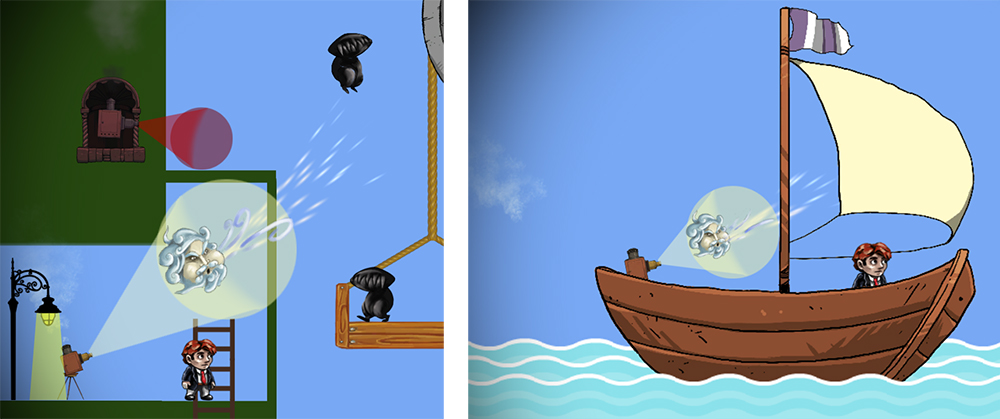
\includegraphics[width= \columnwidth]{images/gameDesign/20_vento.jpg}
	\caption{Utilizzi della proiezione del vento.}
	\label{fig:meccaniche_precinema_vento}
\end{figure}

Esempi di utilizzo delle due meccaniche verranno mostrati nell’analisi dei livelli (riferimento).

Inizialmente si ipotizzava di far utilizzare la lanterna assegnandole uno specifico tasto da tenere premuto. La lanterna sarebbe stata quindi sempre in mano al personaggio ed utilizzata in qualsiasi momento. Tale approccio si sposa perfettamente con alcune proiezioni, come quelle di fantasma ed esca, in quanto l’utente può muovere dinamicamente l’elemento proiettato e direzionarlo in relazione ai movimenti dei nemici, ma impedisce di utilizzare molte delle altre proiezioni teorizzate, in quanto non permette una diretta interazione di queste con il personaggio giocabile.

La soluzione che abbiamo ritenuto più valida è stata quindi quella di permettere al giocatore di poter mirare attraverso la pressione di un tasto, e proiettare al suo rilascio. In questo stesso momento la lanterna magica viene lasciata a terra e continua a proiettare, fino a che il giocatore non decida di riprenderla di nuovo in mano.
Il momento dedicato alla mira, sfrutta l’utilizzo di una sagoma dell’elemento che si andrà a proiettare, così da dare immediatamente al giocatore la sensazione di come e dove verrà creato l’oggetto dello scenario.
Il concetto di mira è stato sviluppato parallelamente all’attuale implementazione di camera e puntatore, in quanto la sagoma dell’oggetto da proiettare compare esattamente nella stessa posizione del puntatore, così da non confondere l’utente con metafore di gioco differenti.
Come si può vedere in Figura~\ref{fig:meccaniche_precinema_swapper}, per tale meccanica ci si è ispirati al videogioco The Swapper (riferimento).

\begin{figure}%[h]
	\centering
	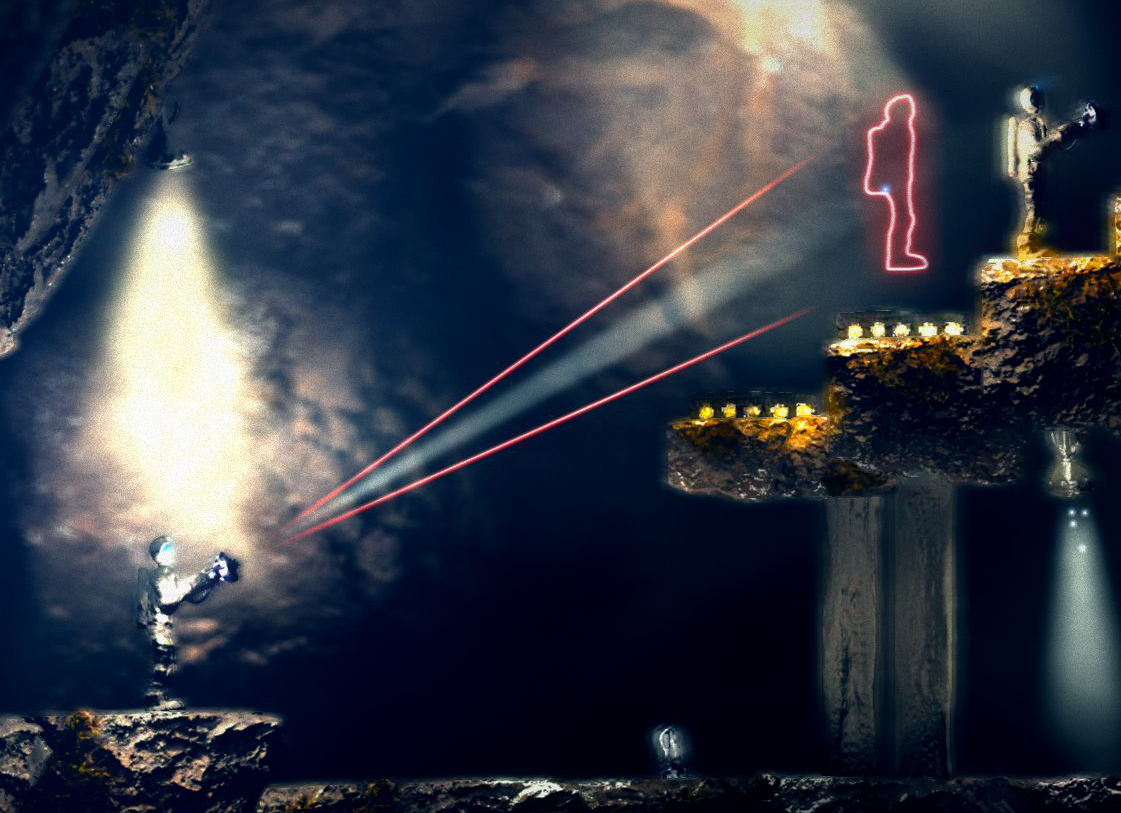
\includegraphics[width= 0.85\columnwidth]{images/gameDesign/21_swapper.jpg}
	\caption{Concetto di mira espresso in The Swapper.}
	\label{fig:meccaniche_precinema_swapper}
\end{figure} 

Un altro elemento di gioco ispirato alla Lanterna Magica è quello che abbiamo definito come \textit{mondo in divenire}.
Come già specificato, la lanterna utilizzava dei vetrini, che potevano anche essere inseriti e rimossi durante gli spettacoli, così da permettere un evolversi delle ambientazioni e di un’eventuale storia da raccontare. Queste operazioni facevano in modo che alcuni elementi apparissero o scomparissero con un effetto di dissolvenza.

Sviluppando perciò il mondo di gioco come se questo fosse un vero spettacolo di lanterna magica, abbiamo ritenuto di poter ottenere un effetto grafico suggestivo e curioso, includendo la possibilità di poter far evolvere lo scenario di gioco con l’apparizione e la scomparsa di elementi in dissolvenza.
Questo processo è stato, in un primo momento, relazionato al raccoglimento di stelle. Il giocatore poteva quindi porsi come obiettivo quello di raggiungere una stella, così da poter far evolvere il mondo di gioco e poter proseguire con il livello.

Dopo un attenta valutazione ed alcuni test effettuati, abbiamo deciso di abbandonare questa strada, anche in relazione all’inserimento di altre tipologie di collezionabili, il cui numero, sommato a quello delle stelle, avrebbe potuto confondere il giocatore per quanto concerne il ruolo di ogni elemento da raccogliere. Inoltre, era presente il rischio che il giocatore avesse dato priorità ad un obiettivo locale, il raccoglimento della stella, e perdere di vista obiettivi più generici di gioco.
Nella attuale implementazione, quindi, l’evoluzione del mondo di gioco è assegnata a dei semplici \textit{trigger} attivati dal passaggio del personaggio (Figura~\ref{fig:meccaniche_precinema_dissolving}). Il posizionamento di tali elementi è chiaramente stato fatto con attenzione e dopo attente fasi di analisi e studio dei livelli.

\begin{figure}%[h]
	\centering
	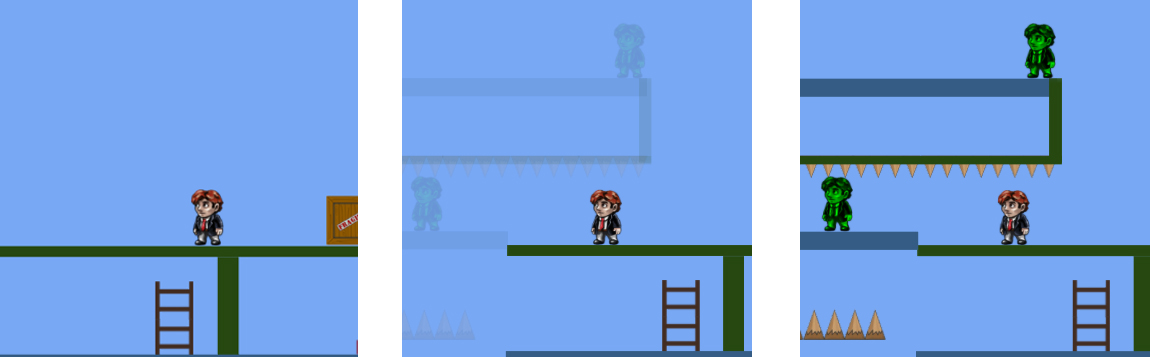
\includegraphics[width= \columnwidth]{images/gameDesign/22.jpg}
	\caption{Meccanica delle Dissolving Views.}
	\label{fig:meccaniche_precinema_dissolving}
\end{figure} 

Le meccaniche di gioco primarie, come abbiamo analizzato, sono quindi quelle \textit{platform} e \textit{puzzle}, enfatizzate dall’utilizzo della Lanterna Magica che permette di interagire ed alterare lo scenario.
Tali elementi di gameplay sono stati però affiancati da altre meccaniche ispirate al contesto del \textit{pre-cinema}.
Tra gli elementi \textit{serious} del nostro videogioco, abbiamo incluso la possibilità di raccogliere degli oggetti e quindi lo sbloccare le relative schede informative che ne descrivono la storia, l’utilizzo ed eventuali curiosità a riguardo (riferimento).

Nei test effettuati (riferimento) abbiamo però notato come i ragazzi fossero poco attratti dall’apertura delle schede informative e quindi dall’apprendere determinati concetti che riteniamo importanti per l’esperienza di gioco e per l’obiettivo di Tesi prefissato.
Abbiamo quindi deciso di inserire diversi elementi aggiuntivi, tra questi alcune meccaniche di gioco, studiate appositamente, per rendere più interessante il raccoglimento di tali oggetti e quindi stimolare curiosità per l’apertura delle relative schede informative.

La camera oscura (riferimento) è un particolare strumento che riproduce all’interno di una delle sue facce, l’immagine capovolta di quanto si trova di fronte al foro della faccia opposta.
Al raccoglimento dell’oggetto relativo perciò, il personaggio si trova in una porzione di gioco già affrontata, per assicurarci che abbia dei riferimenti che non lo facciano trovare spaesato, ma con la camera ruotata di 180 gradi (Figura~\ref{fig:meccaniche_precinema_camera_oscura}). Il giocatore si trova quindi a dover far muovere il personaggio ma facendo attenzione al fatto che i comandi sono invertiti rispetto alla partita svolta fino a quel momento.

\begin{figure}%[h]
	\centering
	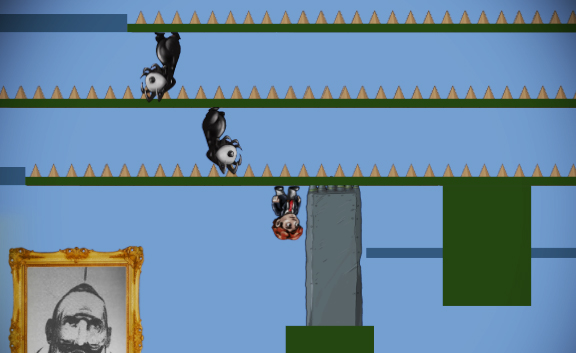
\includegraphics[width= 0.8\columnwidth]{images/gameDesign/23_cameraOscura.jpg}
	\caption{Meccanica della Camera Oscura.}
	\label{fig:meccaniche_precinema_camera_oscura}
\end{figure} 

Al termine di questa breve sezione, viene sbloccata la scheda informativa relativa alla camera oscura, così che l’utente possa informarsi maggiormente nel caso sia abbastanza stimolato a farlo.

Per quanto riguarda le lenti, abbiamo inserito degli approfondimenti che parlano di quelle convergenti e divergenti.
Per far sì che l’oggetto venga contestualizzato all’interno del mondo di gioco, abbiamo studiato un’apposita sezione in cui il personaggio venga rimpicciolito ed ingrandito dal passaggio attraverso delle lenti (Figura~\ref{fig:meccaniche_precinema_lenti}) e si trovi quindi a relazionarsi con elementi di gioco di diverse dimensioni, come delle fessure sui muri, che possono essere affrontati solo se si è passati attraverso la giusta sequenza di lenti.

\begin{figure}%[h]
	\centering
	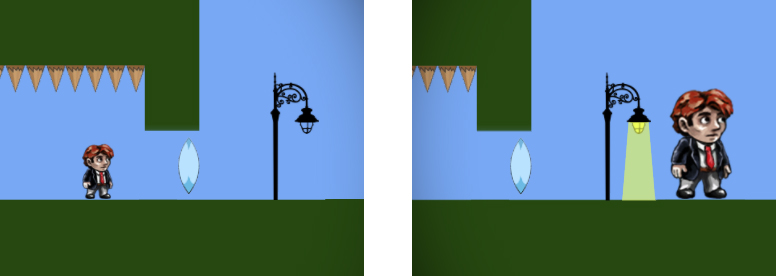
\includegraphics[width= 0.9\columnwidth]{images/gameDesign/24_lenti.jpg}
	\caption{Meccanica delle Lenti.}
	\label{fig:meccaniche_precinema_lenti}
\end{figure} 

Stiamo inoltre valutando la possibilità di includere le suddette meccaniche anche in altre sezioni di gioco. Bisogna sicuramente stare attenti a sfruttarle in maniera intelligente, senza rischiare di esser confusionari e confondere l’utente. Sono state introdotte per stimolare il giocatore ad aprire le schede informative al momento del raccoglimento del relativo oggetto, se dovessero essere inserite in altre sezioni di gioco, dovremmo evitare di avvicinarle ad altri elementi contestualizzanti per non mescolare concetti tra di loro, oltre che usarle con parsimonia per non caricare il giocatore di troppe meccaniche da dover padroneggiare.

\subsection{Elementi di rigiocabilità}
\label{sec:elementi_rigiocabilita}

Con elementi di rigiocabilità vogliamo intendere tutti quei componenti che possono spingere il giocatore a ricominciare livelli di gioco (o il gioco stesso) una volta che questi siano già stati portati a termine.
Nel nostro caso, gli elementi di rigiocabilità più diretti che abbiamo voluto inserire sono le stelle ed i collezionabili. La Figura~\ref{fig:rigiocabilita_stelle_collezionabili} ne mostra degli esempi.

All’interno dei livelli sono presenti degli oggetti che, una volta raccolti, sbloccano la relativa scheda informativa, sono quindi elementi coerenti col contesto, li chiameremo in maniera generica “collezionabili”. Questi sono facilmente raggiungibili dal personaggio principale. Sono generalmente ben visibili e spesso si trovano lungo il percorso primario. Essendo elementi importanti per la componente \textit{serious} del gioco, si vuole evitare che il giocatore li salti per distrazione, ma anzi sia stimolato a raccoglierli e ad informarsi riguardo ciò che ha appena raccolto.

Le stelle sono invece elementi raggiungibili in maniera più difficile, richiedono sempre delle abilità di reazione, di movimento o di ragionamento superiori rispetto ai semplici collezionabili. Il loro unico scopo è quello di permettere l’assoluto completamento del livello.

\begin{figure}%[h]
	\centering
	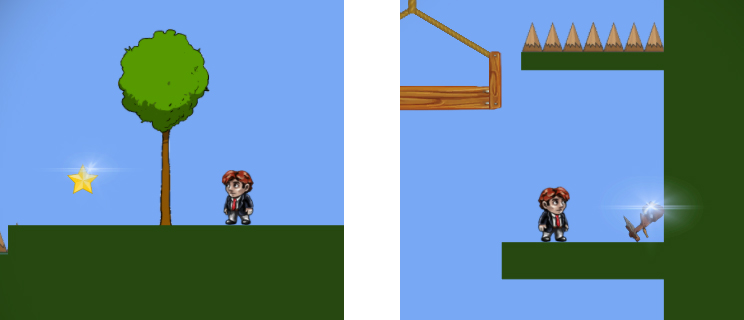
\includegraphics[width= 0.9\columnwidth]{images/gameDesign/25_stelle_collezionabili.jpg}
	\caption{Stelle ed oggetti collezionabili.}
	\label{fig:rigiocabilita_stelle_collezionabili}
\end{figure} 
